\documentclass[essd, manuscript]{copernicus}
\let\unit\undefined
\usepackage{siunitx}

\begin{document}

\title{An ensemble of 48 physically perturbed model estimates of the 1/8\degree{} terrestrial water budget over the conterminous United States, 1980--2015}

\Author[1]{Hui}{Zheng}
\Author[1,2]{Wenli}{Fei}
\Author[3]{Zong-Liang}{Yang}
\Author[3,4]{Jiangfeng}{Wei}
\Author[3,5]{Long}{Zhao}
\Author[3,6]{Lingcheng}{Li}
\Author[7]{Shu}{Wang}

\affil[1]{Key Laboratory of Regional Climate-Environment Research for Temperate East Asia, Institute of Atmospheric Physics, Chinese Academy of Sciences, Beijing, 100029, China}
\affil[2]{University of Chinese Academy of Sciences, Beijing, 100049, China}
\affil[3]{Department of Geological Sciences, John A. and Katherine G. Jackson School of Geosciences, the University of Texas at Austin, Austin, Texas, 78705, USA}
\affil[4]{Collaborative Innovation Center on Forecast and Evaluation of Meteorological Disasters/Key Laboratory of Meteorological Disaster, Ministry of Education/International Joint Research Laboratory on Climate and Environment Change, Nanjing University of Information Science and Technology, Nanjing, 210044, China}
\affil[5]{School of Geographical Sciences, Southwest University, Chongqing, 400715, China}
\affil[6]{Pacific Northwest National Laboratory, Richland, Washington, 99354, USA}
\affil[7]{State Key Laboratory of Operation and Control of Renewable Energy \& Storage Systems, China Electric Power Research Institute, Beijing, 100192, China}

\correspondence{Zong-Liang Yang (\href{mailto:liang@jsg.utexas.edu}{liang@jsg.utexas.edu})}

\runningtitle{NLDAS-NoahMP perturbed-physics ensemble hydrological data}

\runningauthor{Zheng, Fei, Yang, et al.}

\firstpage{1}

\maketitle

\begin{abstract}

Terrestrial water budget (TWB) data over large domains are of high interest for various hydrological applications. Spatiotemporally continuous and physically consistent estimations of TWB rely on land surface models (LSMs). As an augmentation of the operational North American Land Data Assimilation System Phase 2 (NLDAS-2) four-LSM ensemble, this paper describes a dataset simulated from an ensemble of 48 physics configurations of the Noah LSM with multi-physics options (Noah-MP). The 48 Noah-MP physics configurations are selected to give a representative cross-section of commonly used LSMs for parameterizing runoff, atmospheric surface layer turbulence, soil moisture limitation on photosynthesis, and stomatal conductance.

The dataset spans from 1980 to 2015 over the conterminous United States (CONUS) at a monthly temporal resolution and a 1/8\degree{} spatial resolution. The dataset variables include total evapotranspiration and its constituents (canopy evaporation, soil evaporation, and transpiration), runoff (the surface and subsurface components), as well as terrestrial water storage (snow water equivalent, four-layer soil water content from the surface down to 2 m, and the groundwater storage anomaly). The dataset is available at \url{https://doi.org/10.5281/zenodo.7109816} \citep{zheng2022}. Evaluations carried out in this study and previous investigations show that the ensemble performs well in reproducing the observed terrestrial water storage, snow water equivalent, soil moisture, and runoff. Noah-MP complements the NLDAS models well, and adding Noah-MP consistently improves the NLDAS estimations of the above variables in most areas of CONUS\@. Besides, the perturbed-physics ensemble facilities the identification of model deficiencies. The parameterizations of shallow snow, spatially varying groundwater dynamics, and near-surface atmospheric turbulence should be improved in future model versions.

\end{abstract}

\introduction\label{sec:intro}

Estimates of the terrestrial water budgets (TWBs)---evapotranspiration, runoff, terrestrial water storage, and their constituents ---over continental domains are of high interest for a broad range of hydrological applications. Publicly available data have been applied to investigate the state of the terrestrial water cycle \citep{trenberth2013GRL,rodell2015JC, scanlon2018PNASU, yin2020HESS}; to understand the interactions among hydrological processes, vegetation, climate, and human activities \citep{trenberth2013JC,lafontaine2015JAWRA, ward2014PNASU, levia2020NG}; to examine the availability and variability of water resources and use \citep{wu2021JHa, hejazi2014HESS, scanlon2012PNASU, voss2013WRR, lv2019JGRA, le2011PNASU, rodell2009N}; and to assess the risk of extreme events such as droughts \citep{peters-lidard2021BAMS, prudhomme2014PNASU, dai2013NCC, su2021JHa} and floods \citep{emerton2017NC, lin2018JH}.

As the applications have expanded, the availability of TWB estimates has increased rapidly \citep{peters-lidard2018MM, saxe2021HESS, zhang2018HESS}. Commonly used estimation methods include remote sensing, in-situ observations, and model simulations \citep{saxe2021HESS, mccabe2017HESS, pan2012JC, gao2010IJRS, trenberth2007JH}. Among these methods, land surface models (LSMs) are apt for continuously producing physically consistent TWBs over a large domain and long period, and their characteristics are particularly favorable for certain circumstances. For instance, LSMs can estimate various TWB components simultaneously; whereas, for some components, such as runoff \citep{lin2019WRRa, beck2017HESS}, root-zone soil moisture \citep{xia2015JHa, xia2015JH}, and transpiration \citep{lian2018NCC}, direct remote sensing is either unavailable or highly uncertain. Additionally, LSMs are valuable in remote or topographically complex regions because of the sparseness of in-situ observations \citep{kim2021TC}. Estimations based on remote sensing and in-situ observations are often impeded by scale mismatches and observation gaps, whereas these issues are rarely an impairment for LSM simulations. Besides, LSM simulations can complement remote sensing and in-situ observations well. Combinations of estimates from different techniques can improve the estimation accuracy \citep{zhang2018HESS, pan2012JC, zhao2018RSE}, while comparisons between model-simulated estimates and observations can reveal the impacts of human activities \citep{zaussinger2019HESS} and underground processes \citep{zheng2020JAMES}.

Several operational LSM simulation systems have been set up over different regions of the globe \citep{xia2019JMR, shi2011SCES, carrera2015JH, rodell2004BAMS}. The systems combine an ensemble of LSMs to utilize the competitive strengths of different LSMs and eliminate the weakness associated with individual ones. Among them, the North American Land Data Assimilation System (NLDAS) \citep{xia2012JGRAa, xia2012JGRA, mitchell2004JGRA} stands as a pioneering and successful one. The NLDAS phase 2 (NLDAS-2) operates over the conterminous United States (CONUS) from 1979 to near real-time at a spatial resolution of 1/8\degree{}. The system generates a set of multi-source synthesized data of surface meteorology, vegetation, and soils, and uses them to drive an ensemble of four different LSMs. The four LSMs---namely Noah version 2.8 \citep{ek2003JGRA, chen2001MWR, chen2001MWRa, chen1997BM}, Variable Infiltration Capacity (VIC) version 4.0.3 \citep{liang1994JGRA}, Mosaic \citep{koster1992JGRA}, and Sacramento Soil Moisture Accounting (SAC) model \citep{burnash1973}, were selected to give a good cross-section of the diverse range of LSMs \citep{mitchell2004JGRA}. The models have varying strengths and weaknesses in process parameterizations and modeling skills \citep{kumar2017WRR}. A combination of multiple models can produce an aggregated estimate that outperforms most of the individual constituents \citep{fei2021WRR, beck2017HESS, guo2007QJRMS, ajami2007WRR}. An ensemble can also quantify the estimation uncertainty resulting from different model formulations \citep{troin2021WRR, cloke2009JH}. Evaluations of the NLDAS-2 four-LSM ensemble estimates have shown satisfactory performance in matching the observed evapotranspiration (ET) \citep{zhang2020AFM, xia2012JGRA, kumar2018RS}, runoff \citep{xia2012JGRAa}, and soil moisture \citep{xia2015JHa, xia2015JH}.

We have enriched the NLDAS-2 four-model ensemble with 48 perturbed-physics configurations of the Noah LSM with multi-physics options (Noah-MP) \citep{fei2021WRR, zheng2020JAMES, zheng2019WRR}. Noah-MP has more physically realistic representations of vertical stratification than the NLDAS-2 models have. A column of land in Noah-MP consists of a vegetation canopy layer, three snowpack layers, four soil layers, and a groundwater component \citep{niu2011JGRA, yang2011JGRA}. Conceptual (e.g., the five water tanks of SAC) and lumped (e.g., the combined vegetation-soil surface layer of Noah) representations of the stratification of vegetation and soil, as used in the NLDAS-2 models, are minimized. Moreover, Noah-MP has a more comprehensive representation of various land surface processes that are evident at different depths. The modeled processes include snow accumulation and ablation, infiltration, percolation, retention, freeze-thaw of snow or soil water, groundwater recharge/discharge, and energy constraints \citep{niu2011JGRA}. These improvements in vertical stratification and process parameterizations are expected to better estimate TWBs. Indeed, previous comparisons between Noah-MP and the four NLDAS-2 LSMs have shown that Noah-MP is comparable or better when it comes to estimating soil moisture \citep{cai2014JGRAa}, runoff \citep{cai2014JGRA, fei2021WRR}, and ET \citep{zhang2020AFM}.

Our enrichment also features a single-model perturbed-physics ensemble, which is different from the widely used multi-model ensemble approach. The Noah-MP ensemble is constructed by shuffling the available parameterization options of several selected processes. The ensemble size grows exponentially as a multiplication of the available parameterization options of different processes \citep{yang2011JGRA, zhang2016JGRA, gan2019WRR}. A large ensemble should give a broad cross-section of feasible model formulations to account for the model uncertainty in TWB estimation \citep{telteu2021GMD, mitchell2004JGRA} and is critical for a statistically reliable estimation of the probability of hydrological events such as floods and droughts \citep{troin2021WRR}. The single-model perturbed-physics ensemble also facilitates uncertainty attribution and reduction. The ensemble consists of pairs that are different in the parameterization of one process and the same for another. Variance analysis of the ensemble can quantify the contribution of the parameterization of a process and compare the relative importance of two processes \citep{zheng2019WRR, clark2011WRR}. Such quantification could inform further model development to reduce the model uncertainty. However, there are also pitfalls unique to the single-model perturbed-physics ensemble. \citet{fei2021WRR} found that the ensemble members generated by naive perturbation of the Noah-MP physics are not independent enough from each other. The low independence hinders the skill gained from the ensembling method. The finding suggests that advanced techniques of physics perturbations should be developed to maximize the ensemble skill and minimize the ensemble size. An open-accessible dataset should facilitate the research that leverages the advantages and addresses the issues of the perturbed-physics ensemble.

We have previously evaluated the runoff and compared it with NLDAS-2 \citep{fei2021WRR}. This paper describes the estimation of all the TWB variables, along with the description of the spread among the ensemble members, the difference with the NLDAS models, and the performance with reference to various observations are presented. The paper is organized as follows. Section~\ref{sec:data} presents the information necessary for using the dataset, including the dataset variables, file organization, and the source data and models used for data generation. Section~\ref{sec:methods} describes the intercomparison methods, evaluation metrics, and reference datasets. Section~\ref{sec:results} presents the results and discussion. Finally, after stating the data availability in Section~\ref{sec:availability}, Section~\ref{sec:conclusions} draws conclusions.

\section{Data description}\label{sec:data}

The dataset contains gridded water budget variables over CONUS\@. Section~\ref{sec:data:variables} describes the dataset variables and their physical relationships. The 48 Noah-MP physics configurations used to create the dataset are detailed in Section~\ref{sec:data:noahmp}. Section~\ref{sec:data:static} brief the atmospheric forcing, static parameters of vegetation and soil, and simulation settings.

\subsection{Dataset variables}\label{sec:data:variables}

Table~\ref{tab:variables} lists the dataset variables. The variables are available at each 1/8\degree{} grid point in NLDAS-2, indicated by a land-water mask (\(X\)). The surface water budgets of each grid cell are represented as follows:

\begin{table}[t]
  \caption{The dataset variables.}
  \label{tab:variables}
  \begin{tabular}{lll}
  \tophline
  Symbol         & Units                   & Description \\
  \middlehline
  \multicolumn{3}{c}{surface water budget} \\
  \(E\)          & \unit{kg.m^{-2}.s^{-1}} & total evapotranspiration \\
  \(E_{can}\)    & \unit{kg.m^{-2}.s^{-1}} & evaporation of canopy interception \\
  \(E_{gnd}\)    & \unit{kg.m^{-2}.s^{-1}} & direct evaporation from the ground \\
  \(E_{tran}\)   & \unit{kg.m^{-2}.s^{-1}} & transpiration \\
  \(R\)          & \unit{kg.m^{-2}.s^{-1}} & total runoff \\
  \(R_{srf}\)    & \unit{kg.m^{-2}.s^{-1}} & surface runoff \\
  \(R_{und}\)    & \unit{kg.m^{-2}.s^{-1}} & subsurface runoff \\
  \(W\)          & \unit{kg.m^{-2}}        & terrestrial water storage \\
  \(W_{snow}\)   & \unit{kg.m^{-2}}        & snow water equivalent \\
  \(W_{gw}\)     & \unit{kg.m^{-2}}        & groundwater storage \\
  \(w_{soil,i}\) & \unit{m^3.m^{-3}}       & volumetric soil water content \\
  \(z_{snow}\)   & \unit{m}                & snow depth \\
  [1pt]
  \multicolumn{3}{c}{auxiliary variables} \\
  \(X\)          & -                       & land-water mask \\
  \bottomhline
\end{tabular}

\end{table}

Neglecting horizontal water exchange between adjacent grids, the water budget closure can be obtained among the precipitation (\(P\), \unit{kg.m^{-2}.s^{-1}}), ET (\(E\)), runoff (\(R\)), and terrestrial water storage change (\(W'=\frac{dW}{dt}\), \unit{kg.m^{-2}.s^{-1}}) \citep{zheng2020JAMES}:
\begin{equation}
  P = E + R + W'
  \text{,}
\end{equation}
where precipitation (\(P\)) is from NLDAS-2 (described in Section~\ref{sec:intro}) and used as the model input.

Noah-MP resolves the components of the water budget closure equation (1). ET (\(E\)) consists of canopy evaporation (\(E_{can}\)), ground evaporation (\(E_{gnd}\)), and transpiration (\(E_{tran}\)):
\begin{equation}
  E = E_{can} + E_{gnd} + E_{tran}
  \text{.}
\end{equation}
Runoff (\(R\)) has a surface (\(R_{srf}\)) and subsurface (\(R_{sub}\)) component:
\begin{equation}
  R = R_{srf} + R_{sub}
  \text{.}
\end{equation}
Terrestrial water storage (TWS, \(W\)) is the sum of snow water equivalent (SWE, \(W_{snow}\)), groundwater storage in unconfined aquifers (\(W_{gw}\)), and soil water content in the four model layers (\(W_{soil,i}\)):
\begin{equation}
  W = W_{snow} + W_{gw} + \sum_{i=1}^{N_{soil}} W_{soil,i}
  \text{,}
\end{equation}
where \(N_{soil} = 4\) is the number of soil layers. Soil water storage (\(W_{soil,i}\)) is not included in the dataset but can be calculated from the volumetric water content (\(w_{soil,i}\)) as follows:
\begin{equation}
  W_{soil,i} = \rho_{wat} w_{soil,i} \Delta z_{soil,i} \quad \mathrm{for}\ i = 1, \cdots, N_{soil}
  \text{,}
\end{equation}
where \(\rho_{wat} = \qty{1000}{kg.m^{-3}}\) is the water density; and \(\Delta z_{soil,1} = \qty{0.1}{m}\), \(\Delta z_{soil,2} = \qty{0.3}{m}\), \(\Delta z_{soil,3} = \qty{0.6}{m}\), and \(\Delta z_{soil,4} = \qty{1}{m}\) are the thicknesses of the four soil layers.

\subsection{The 48 Noah-MP physics configurations}\label{sec:data:noahmp}

The Noah-MP LSM version 3.6 is used. We perturbed the parameterization of runoff, stomatal conductance, soil moisture stress factor, and near-surface atmospheric turbulence. The processes are selected as they directly control runoff generation and evapotranspiration. Their importance has been shown in global simulations \citep{yang2011JGRA}. The perturbation creates an ensemble of 48 members (48 = 4 runoff \times{} 2 stomatal conductance \times{} 3 soil moisture stress \times{} 2 turbulence). Limited by computational resources, we did not perturb the parameterization of the cryosphere hydrological processes such as snow albedo \citep{chen2014JGRA,he2019JGRA} and rain-snow partitioning \citep{wang2019GRL}, which may limit the usage of the dataset in cryosphere hydrology. Appendix~\ref{sec:app:noahmp} details the formulation of and parameters in the selected parameterization. The parameters use the Noah-MP default values.

\subsection{Domain, temporal span, atmospheric forcings, and static parameters}\label{sec:data:static}

The simulation domain covers the CONUS (25\degree{}--53\degree{}N, 125\degree{}--67\degree{}W) at a spatial resolution of 0.125\degree{}.

The hourly NLDAS-2 atmospheric forcings were used to drive the 48 Noah-MP configurations. This study used seven forcing variables: downward solar radiation, downward longwave radiation, air temperature, surface pressure, specific humidity, wind speed, and precipitation rate. The static datasets, including topography (\url{https://ldas.gsfc.nasa.gov/nldas/elevation}), predominant vegetation class (\url{https://ldas.gsfc.nasa.gov/nldas/vegetation-class}), and soil texture type (\url{https://ldas.gsfc.nasa.gov/nldas/soils}), are also the same as those in NLDAS-2. We used the default Noah-MP lookup tables to convert the input vegetation and soil types to parameter values.

The simulation spans 36 years from January 1980 to December 2015 at a time step of 15 minutes. The initial states on 1 January 1980 were obtained by cycling the year 1979 one hundred times.

\section{Intercomparison and evaluation methods}\label{sec:methods}

The evaluations and intercomparisons in this paper are performed for twelve River Forecast Centers (RFCs): Northeast (NE), Mid-Atlantic (MA), Ohio (OH), Lower Mississippi (LM), Southeast (SE), North Central (NC), Northwest (NW), Arkansas (AB), Missouri (MB), West Gulf (WG), California-Nevada (CN), and Colorado (CB). Figure S1 displays the geographical delineation of the RFCs. More details on the RFCs, such as their multi-year average precipitation, potential evaporation, and topography, can be found in \citet[Figure 1]{fei2021WRR}.

The intercomparison and evaluations were conducted at different time scales---the long-term climatological mean, annual cycle, and interannual anomaly. Section~\ref{sec:methods:variation} details how the temporal variations and ensemble spread are derived for the time scales. We utilized the Taylor diagram and Taylor Skill Score (TSS) to measure the performance of Noah-MP against various reference datasets. The evaluation methods are shown in Section~\ref{sec:methods:taylor}, and the reference datasets are described in Section~\ref{sec:methods:ref}. In addition to the inter-comparisons and evaluations, Section~\ref{sec:methods:sobol} introduces the Sobol' sensitivity index for the process sensitivity analysis.

\subsection{Temporal variability and ensemble spread}\label{sec:methods:variation}

We calculated the total temporal variability (\(\sigma_{total}\)), the variability of the annual cycle (\(\sigma_{ancy}\)), and the interannual variability (\(\sigma_{anom}\)) for each ensemble member and the ensemble arithmetic mean following \citet{dirmeyer2006BAMS}:
\begin{align}
  \sigma_{total} & = \sqrt{\frac{1}{12 Y}\sum_{y,m} (x_{y,m} - x_{clim})^2}
  \text{,}
  \label{eq:var:total} \\
  \sigma_{ancy}  & = \sqrt{\frac{1}{12}\sum_{m} (x_{ancy,m} - x_{clim})^2}
  \text{,} \\
  \sigma_{anom}  & = \sqrt{\frac{1}{12 Y} \sum_{y,m} (x_{y,m} - x_{ancy,m})^2}
  \text{,}
\end{align}
where \(x_{clim}\), \(x_{ancy}\), and \(x_{anom}\) are the climatology, annual cycle, and interannual anomaly of the monthly time series \(x_{y,m}\) (month \(m\) of the year \(y\); \(m=1, \cdots, 12\); \(y=1, \cdots, Y\)).

The ensemble spread for the total time series (\(\check{\sigma}_{total}\)), annual cycle (\(\check{\sigma}_{ancy}\)), and interannual anomaly (\(\check{\sigma}_{anom}\)) are derived also following \citet{dirmeyer2006BAMS}:
\begin{align}
  \check{\sigma}_{total} & = \frac{1}{T} \sum_{t=1}^{T} \sigma(x_{y,m})
  \text{,} \\
  \check{\sigma}_{ancy}  & = \frac{1}{12} \sum_{m=1}^{12} \sigma(x_{ancy})
  \text{,} \\
  \check{\sigma}_{anom}  & = \frac{1}{12Y} \sum_{y=1}^{Y} \sum_{m=1}^{12} \sigma(x_{anom})
  \text{,}
\end{align}
where \(\sigma(x) = \sqrt{[\sum_{n=1}^{N}(x-\check{x})^2]/N}\) denotes the standard deviation across the ensemble members at each time step. \(\check{x}\) denotes the arithmetic ensemble mean.

We calculated the ratio (\(r=\check{\sigma}/\sigma\)) of ensemble spread \(\check{\sigma}\) to temporal variability \(\sigma\) for the total monthly time series (with a subscript of ``total''), annual cycle (``ancy''), and interannual anomaly (``anom''). The ratio enables the intercomparison of the ensemble spread among the selected time scales. A grade is assigned according to the ratio following \citet{dirmeyer2006BAMS}: a grade ``A'' for \(r < 0.316\); ``B'' for \(0.316 \le r < 1\); ``C'' for \(1 \le r < 3.16\); ``D'' for \(3.16 \le r < 10\); and ``E'' for \(r > 10\). A lower (higher) \(r\) or a higher (lower) grade denotes a lower (higher) ensemble spread.

\subsection{Taylor diagram and skill score}\label{sec:methods:taylor}

The Taylor diagram \citep{taylor2001JGRA} is a graphical representation of how closely a model simulation matches observations in terms of correlation coefficient (\(R\)), normalized unbiased root-mean-square error (nuRMSE), and normalized standard deviation (\(\hat{\sigma}_{f}\)). The TSS is an index that measures the distance between a model simulation and the observations in the Taylor diagram. The TSS is defined as follows:
\begin{align}
  TSS              & = \frac{4 (1 + R)}{(\hat{\sigma}_{f} + \frac{1}{\hat{\sigma}_{f}})^2 ( 1 + R_{0})} \\
  \hat{\sigma}_{f} & = \frac{\sigma_{f}}{\sigma_{o}}
\end{align}
where \(\sigma_{f}\) and \(\sigma_{o}\) are the standard deviations of the model simulation and the observation, and \(R_{0}\) is the maximum correlation coefficient attainable (in this study, \(R_{0} = 1\)). The value range of TSS is from 0 to 1. A higher TSS indicates a higher overall performance of model prediction with reference to the observations.

\subsection{Sobol's total sensitivity index}\label{sec:methods:sobol}

The sensitivity of the Noah-MP ensemble to a physical process can be quantified by the Sobol' total sensitivity index \citep{sobol1993MMCE, zheng2019WRR}. The Sobol' total sensitivity index measures the proportion of the variance of different processes to the total variance, which is defined as follows:
\begin{equation}
  S_{\Lambda} = \frac{\mathrm{E}_{\sim\Lambda}(\mathrm{Var}_{\Lambda}(Y|\sim\Lambda))}{\mathrm{Var}(Y)}
  \text{,}
\end{equation}
where \(S_{\Lambda}\) is the Sobol' total sensitivity index for one process \(\Lambda\); \(\sim\Lambda\) represents the other processes except for \(\Lambda\); \(Y\) represents the 48 Noah-MP ensemble members; \(\mathrm{Var}(Y)\) is the variance of \(Y\); \(\mathrm{Var}_{\Lambda}(Y|\sim\Lambda)\) denotes the variance among different parameterization schemes of the process \(\Lambda\), and \(\mathrm{E}(\sim\Lambda)\) denotes the arithmetic average across all combinations of the other processes except for \(\Lambda\). Detailed calculations and examples can be found in \citet[Appendix A]{zheng2019WRR}.

\subsection{Reference data}\label{sec:methods:ref}

\subsubsection{Terrestrial water storage}\label{sec:methods:ref:tws}

We used the 1\degree{}\times{}1\degree{} monthly Gravity Recovery and Climate Experiment (GRACE) land water-equivalent-thickness surface mass anomaly, level-3, Release 6.0, version 04, as the reference of TWS (\(W\) in Table~\ref{tab:variables}). The GRACE products from different processing centers are slightly different. To reduce the noise of the estimates \citep{sakumura2014GRL}, we used the arithmetic average of the products from three centers: (1) GeoForschungsZentrum Potsdam (or the German Research Center for Geosciences) (\url{https://podaac.jpl.nasa.gov/dataset/TELLUS_GRAC_L3_GFZ_RL06_LND_v04}), (2) the Center for Space Research at the University of Texas, Austin (\url{https://podaac.jpl.nasa.gov/dataset/TELLUS_GRAC_L3_CSR_RL06_LND_v04}), and (3) NASA's Jet Propulsion Laboratory (\url{https://podaac.jpl.nasa.gov/dataset/TELLUS_GRAC_L3_JPL_RL06_LND_v04}). The GRACE satellites began orbiting Earth on 17 March 2002. We selected the period from 2003 to 2015 for the evaluation. There are fourteen missing values during the period, which were filled with a simple linear interpolation.

The GRACE products experience signal leakages between land and water \citep{save2016JGRSE}. Such signal leakage could impact the estimation in the RFCs that are adjacent to the Great Lakes \citep{ma2017JGRA} and oceans. To alleviate the impacts of the Great Lakes, we corrected the GRACE TWS estimates in the NC, OH, and NE RFCs using the water level variations observed by the National Oceanic and Atmospheric Administration (NOAA). Appendix~\ref{app:tws} details the algorithm.

\subsubsection{Soil moisture}\label{sec:methods:ref:sm}

We used the daily North American Soil Moisture Database (NASMD, \url{http://soilmoisture.tamu.edu}) \citep{quiring2016BAMS} as the reference for the simulated soil moisture (\(W_{soil,i}\) in Table~\ref{tab:variables}), similar to previous NLDAS evaluations \citep{xia2015JHa, xia2015JH}. NASMD assembles the soil moisture time series at multiple depths of more than 2200 stations of 24 networks with quality control. The observation depth varies with the network. We interpolated the observations to the centers of the Noah-MP soil layers, which are \qty{0.05}{m}, \qty{0.25}{m}, \qty{0.7}{m}, and \qty{1.5}{m}, respectively. The interpolation is performed only when a valid observation is exactly at, or two valid observations exist above and below, the given depth; otherwise, a missing value is given. We excluded the soil layers with more than 50\% missing values to minimize the impacts of missing values on the evaluation, after which 264 \(w_{soil,1}\), 214 \(w_{soil,2}\), 95 \(w_{soil,3}\), and 23 \(w_{soil,4}\) valid time series remained. Daily data from 1996 to 2013 were then aggregated into monthly values. For any month, if less than 10 days of valid data is available, a missing value is assigned.

\subsubsection{Snow water equivalent}

We used the daily Snow Data Assimilation System (SNODAS, \url{https://nsidc.org/data/G02158/versions/1}) as the reference of SWE (\(W_{snow}\) in Table~\ref{tab:variables}). SNODAS is a data assimilation system developed by the NOAA National Weather Service's National Operational Hydrologic Remote Sensing Center. This system aims to provide a physically consistent framework to combine snow modeling and observations from satellites, airborne platforms, and ground stations (National Operational Hydrologic Remote Sensing Center, 2004). The original spatial resolution is 1\,km\times{}1\,km, and we aggregated the data to the 0.125\degree{} NLDAS grids. SNODAS began on 2003-09-28, and we selected the period from September 2004 to August 2015 that spans eleven whole snow seasons. \citet{clow2012HP} showed that the SNODAS SWE performs well in the forest areas of the Colorado Rocky Mountains, but performs poorly in the alpine areas.

\subsubsection{Evapotranspiration}\label{sec:methods:ref:et}

We used plot-scale AmeriFlux observations and two gridded products as the reference ET (\(E\) in Table\ref{tab:variables}). The two gridded products are derived from different methods, and a common evaluation period from 1982 to 2015 is selected for this study. The gridded products have different spatial resolutions. We downscaled the data to the NLDAS grids and then aggregated them to the 12 RFCs.

We selected 25 AmeriFlux sites (\url{https://ameriflux.lbl.gov}). The 25 selected sites were selected because they have the longest observation periods for seven major land cover types (i.e., evergreen forest, deciduous forest, mixed forest, shrubland, savanna, grassland, and cropland). Figure S1 and Table S1 detail the selected sites. The data have been widely used in LSM evaluations \citep{cai2014JGRA, zhang2020AFM}. AmeriFlux provides hourly or half-hourly latent heat measurements. We converted the measurement to ET by dividing the latent heat of water vaporization (\qty{2.5104e6}{J.kg^{-1}}). The hourly or half-hourly ET is then aggregated into monthly values. In the process of aggregation, if there were less than eight valid hours in a day, a missing day was marked; if there were fewer than ten valid days in a month, a missing month was assigned; if there was less than 50\% valid months, the time series was dropped. In this study, the data serve as the ground truth for the gridded ET products and model estimation.

The first gridded ET product is FLUXNET Multi-Tree Ensemble (MTE) \citep{jung2009B} (\url{https://www.bgc-jena.mpg.de/geodb/projects/Home.php}). FLUXNET MTE ET is a monthly data produced from the FLUXNET eddy covariance measurements, remote sensing, and meteorological data using the multi-tree ensemble statistical method \citep{jung2009B}. The product is widely used in LSM evaluations \citep{cai2014JGRA, ma2017JGRA, xia2016JGRA, jung2019SD, fang2020AFM, zhang2020AFM, pan2020HESS}. FLUXNET MTE ET has a spatial resolution of 0.5\degree{}\times{}0.5\degree{}. We remap the data to the 0.125\degree{}\times{}0.125\degree{} NLDAS grids with a first-order conservative method. We use the FLUXNET ET as the reference for the annual cycle since it replicates the AmeriFlux observations best among the two gridded products (Table~S2--S4).

The second gridded ET product is the Global Land Evaporation Amsterdam Model (GLEAM), version 3.3a (\url{https://www.gleam.eu}), which is another widely used ET product \citep{xu2019JHa}. GLEAM estimates transpiration, canopy evaporation, soil evaporation, open-water evaporation, and sublimation separately, and then sums them as ET\@. The method aims to maximize the utilization of satellite information. The product estimates monthly ET at a spatial resolution of 0.25\degree{}\times{}0.25\degree{}. We bilinearly interpolated the data to the NLDAS grids. The GLEAM ET is used as the reference for the interannual anomaly as it better replicates the AmeriFlux-observed anomaly than FLUXNET (Table~S2--S4).

\subsection{NLDAS ensemble}\label{sec:methods:nldas}

We used three NLDAS-2 models---namely Noah-2.8, VIC-4.0.3, and Mosaic, as the benchmark of the Noah-MP ensemble. Their outputs can be publicly downloaded from the NASA Goddard Earth Sciences Data and Information Services Center (\url{https://disc.gsfc.nasa.gov/datasets?keywords=NLDAS}). More information on the NLDAS-2 models, the forcing and static datasets, and simulation settings can be found in \citet{xia2012JGRA, xia2012JGRAa}. The NLDAS-2 datasets have been proven to perform soundly for regional hydrological simulations \citep{xia2012JGRA, xia2012JGRAa, xia2016JGRA, xia2015JHa, xia2015JH} and are widely used as a benchmark for LSM evaluations \citep{cai2014JGRAa, fei2021WRR}.

\section{Results and discussions}\label{sec:results}

In this section, we begin by intercomparing the ensemble spread of the dataset variables (Section~\ref{sec:results:spread}). Then, Sections~\ref{sec:results:twsa}--\ref{sec:results:et} examine the performance and ensemble spread of the TWS anomaly (TWSA), SWE, soil moisture, and ET, in comparison with the NLDAS ensemble. The performance of runoff can be found in our previous paper \citet{fei2021WRR} and \citet{zheng2020JAMES}.

\subsection{Comparison of the ensemble spread}\label{sec:results:spread}

\begin{table*}[t]
  \caption{The climatological mean, ensemble spread, and temporal variability of different dataset variables. \(\bar{\check{x}}\) denotes the climatological average of the ensemble mean. \(\check{\sigma}_{ancy}\), \(\check{\sigma}_{anom}\), and \(\check{\sigma}_{total}\) denote the spread of the 48 Noah-MP configurations in simulating the multi-year averaged annual cycle, interannual anomaly, and total 36-year monthly time series, respectively. \(\sigma_{ancy}\), \(\sigma_{anom}\), and \(\sigma_{total}\) denote the temporal variability of the annual cycle, interannual anomaly, and the total time series, respectively. The rating of the ratio \(\check{\sigma}/\sigma\) is defined in Section~\ref{sec:methods:variation}. The units of the variables are presented in Table~\ref{tab:variables}. \(\tilde{W}\) (\(\tilde{W}_{gw}\)) denotes the terrestrial water storage (groundwater) anomaly (\unit{kg.m^{-2}}), whereas \(W'\) (\(W'_{gw}\)) denotes the monthly terrestrial water storage (groundwater) change (\unit{kg.m^{-2}.s^{-1}}).}
  \label{tab:statistics}
  \begin{tabular}{lcccccccccccc}
    \tophline
    \multirow{2}{*}{Variables} & \multicolumn{3}{c}{Ensemble Spread} & \multicolumn{3}{c}{Temporal Variability} & \multicolumn{3}{c}{\(R\)} & \multicolumn{3}{c}{Rating}                                                                                                             \\
                      & \(\sigma_{lss,ancy}\) & \(\sigma_{lss,anom}\) & \(\sigma_{lss,total}\) & \(\sigma_{ancy}\) & \(\sigma_{anom}\) & \(\sigma_{ancy}\) & \(R_{ancy}\) & \(R_{anom}\) & \(R_{total}\) & ancy & anom & total \\
    \middlehline
    \(E\)             & \num{1.1938e-6}       & \num{2.6612e-7}       & \num{1.2223e-6}        & \num{1.1764e-5}   & \num{1.1842e-6}   & \num{1.1823e-5}   & \num{0.1015} & \num{0.2247} & \num{0.1034}  & A    & A    & A     \\
    \(E_{can}\)       & \num{2.0698e-7}       & \num{4.1702e-8}       & \num{2.0699e-7}        & \num{1.1083e-6}   & \num{3.0769e-7}   & \num{1.1502e-6}   & \num{0.1868} & \num{0.1355} & \num{0.1800}  & A    & A    & A     \\
    \(E_{gnd}\)       & \num{7.3255e-7}       & \num{1.4349e-7}       & \num{7.4295e-7}        & \num{3.6413e-6}   & \num{7.7774e-7}   & \num{3.7235e-6}   & \num{0.2012} & \num{0.1845} & \num{0.1995}  & A    & A    & A     \\
    \(E_{tran}\)      & \num{1.3345e-6}       & \num{2.0629e-7}       & \num{1.3483e-6}        & \num{7.8742e-6}   & \num{6.6551e-7}   & \num{7.9023e-6}   & \num{0.1695} & \num{0.3100} & \num{0.1706}  & A    & A    & A     \\
    \(R\)             & \num{1.2233e-6}       & \num{3.6872e-7}       & \num{1.2591e-6}        & \num{3.1335e-6}   & \num{3.6872e-7}   & \num{1.2591e-6}   & \num{0.3904} & \num{0.2061} & \num{0.3490}  & B    & A    & B     \\
    \(R_{srf}\)       & \num{6.8201e-7}       & \num{2.2459e-7}       & \num{7.0071e-7}        & \num{6.9029e-7}   & \num{5.7802e-7}   & \num{9.0033e-7}   & \num{0.9880} & \num{0.3885} & \num{0.7783}  & B    & B    & B     \\
    \(R_{sub}\)       & \num{1.0013e-6}       & \num{3.4277e-7}       & \num{1.0389e-6}        & \num{2.4692e-6}   & \num{1.3121e-6}   & \num{2.7962e-6}   & \num{0.4055} & \num{0.2612} & \num{0.3712}  & B    & A    & B     \\
    \(W'\)            & \num{5.5732}          & \num{3.4333}          & \num{6.4796}           & \num{44.9508}     & \num{18.0598}     & \num{48.4430}     & \num{0.1240} & \num{0.1901} & \num{0.1338}  & A    & A    & A     \\
    \(\Delta W\)      & \num{2.8444}          & \num{0.8990}          & \num{2.9549}           & \num{22.5839}     & \num{5.9302}      & \num{23.3270}     & \num{0.1259} & \num{0.1516} & \num{0.1267}  & A    & A    & A     \\
    \(W'_{gw}\)       & \num{0.6713}          & \num{0.8549}          & \num{1.0856}           & \num{8.1760}      & \num{6.1079}      & \num{10.1988}     & \num{0.0821} & \num{0.1400} & \num{0.1064}  & A    & A    & A     \\
    \(\Delta W_{gw}\) & \num{0.3742}          & \num{0.3005}          & \num{0.4812}           & \num{4.1177}      & \num{1.6318}      & \num{4.4243}      & \num{0.0909} & \num{0.1842} & \num{0.1088}  & A    & A    & A     \\
    \(W_{snow}\)      & \num{0.1254}          & \num{0.1273}          & \num{0.1726}           & \num{7.5644}      & \num{3.8036}      & \num{8.4669}      & \num{0.0166} & \num{0.0335} & \num{0.0204}  & A    & A    & A     \\
    \(w_{soil,1}\)    & \num{0.0066}          & \num{0.0009}          & \num{0.0067}           & \num{0.0242}      & \num{0.0102}      & \num{0.0262}      & \num{0.2726} & \num{0.0933} & \num{0.2537}  & A    & A    & A     \\
    \(w_{soil,2}\)    & \num{0.0084}          & \num{0.0012}          & \num{0.0085}           & \num{0.0194}      & \num{0.0081}      & \num{0.0210}      & \num{0.4337} & \num{0.1522} & \num{0.4040}  & B    & A    & B     \\
    \(w_{soil,3}\)    & \num{0.0119}          & \num{0.0018}          & \num{0.0121}           & \num{0.0227}      & \num{0.0088}      & \num{0.0244}      & \num{0.5251} & \num{0.2080} & \num{0.4958}  & B    & A    & B     \\
    \(w_{soil,4}\)    & \num{0.0146}          & \num{0.0018}          & \num{0.0147}           & \num{0.0160}      & \num{0.0071}      & \num{0.0175}      & \num{0.9110} & \num{0.2594} & \num{0.8394}  & B    & A    & B     \\
    \bottomhline
\end{tabular}

\end{table*}

We aggregated the dataset variables across CONUS\@. Table~\ref{tab:statistics} summarizes the ensemble spread and temporal variability of the ensemble mean for all the dataset variables. Among the variables, runoff (including surface and subsurface components) shows the largest spread, accounting for one-fifth to one-third of the climatological mean. The ensemble spread is comparable to or larger than the temporal variability. The magnitude is similar to that estimated in GSWP-2. The spread of ET and TWS is significantly smaller than those observed in GSWP-2. The high consistency among the Noah-MP configurations could be a sign of the limited sampling of available process parameterizations but also could be a result of continuous model improvements. ET might be the former case since the ensemble does not perturb several important processes such as roughness sublayer \citep{abolafia-rosenzweig2021JAMES} and plant hydraulics \citep{li2021JAMESa}. TWS is likely the latter case since the parameters of different groundwater schemes are calibrated using GRACE \citep{niu2007JGRa}. The spread of snow water equivalent depicts the smallest spread, which is 2.5\% of the climatological mean. The small spread reflects a limited sampling of the cryosphere processes as discussed in Section~\ref{sec:data:noahmp}. For soil moisture, the ensemble spread is marginal at the surface and increases significantly in the deep layers. The difference hints that the controlling processes vary with depth. The surface soil moisture is tightly controlled by the atmospheric forcings, whereas the spread of the sub-surface soil moisture hints at the complex interplay among various land surface processes (e.g., root water uptake and subsurface runoff) \citep{koster2015BAMS}.

Table~\ref{tab:statistics} also shows the comparison between the annual cycle and interannual anomaly for different variables. For runoff and soil moisture, the ensemble spread in the annual cycle is larger (i.e., \(\check{\sigma}_{ancy} \ge \sigma_{anom}\)). Whereas for transpiration (\(E_{tran}\)), groundwater storage (\(\hat{W}_{gw}\) and \(W'_{gw}\)), and snow water equivalent (\(W_{snow}\)), the spread is larger for the interannual anomaly (i.e., \(\check{\sigma}_{ancy} \le \sigma_{anom}\)). The dynamics at different times are modulated by different processes \citep{dickinson2003AAS}. Since the time scale of the interannual anomaly is smaller than that of the annual cycle, the land surface memory and the associated land model parameterizations may contribute a larger part to the annual cycle, whereas the interannual anomaly is more tightly controlled by atmospheric forcing. The smaller ensemble spread in the annual cycle than in the interannual anomaly is a sign of insufficient representation of the physics uncertainty.

\subsection{Terrestrial water storage anomaly}\label{sec:results:twsa}

\begin{figure*}[t]
  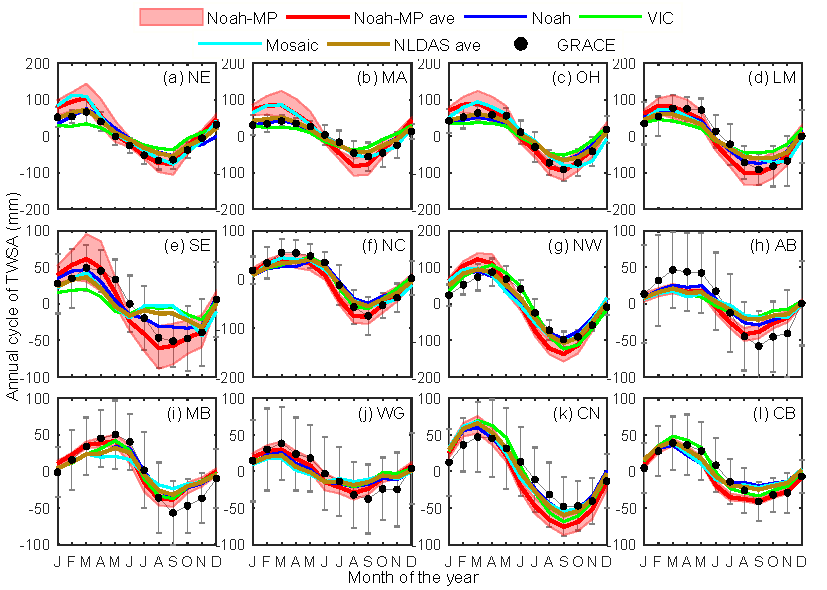
\includegraphics[width=12cm]{fig/fig01.pdf}
  \caption{Annual cycle of TWSA from the model estimates and GRACE in the 12 RFCs for the period 2003--2015. The TWSA is calculated from the monthly TWS by subtracting the 13-year average (2003 to 2015). Black dots denote the GRACE observations. Error bars show the standard deviation of the year-to-year differences. The shaded areas denote the range between the maxima and minima of the 48 Noah-MP estimates. The solid red line denotes the Noah-MP multi-physics ensemble mean. The three NLDAS models (Noah, Mosaic, VIC) and their ensemble mean are denoted by the blue, green, cyan, and dark golden lines, respectively. The twelve RFCs are sorted based on climatic aridity, i.e., the most humid RFC in the top left and the driest RFC in the bottom right.}
  \label{fig:twsa:ancy}
\end{figure*}

\begin{figure*}[t]
  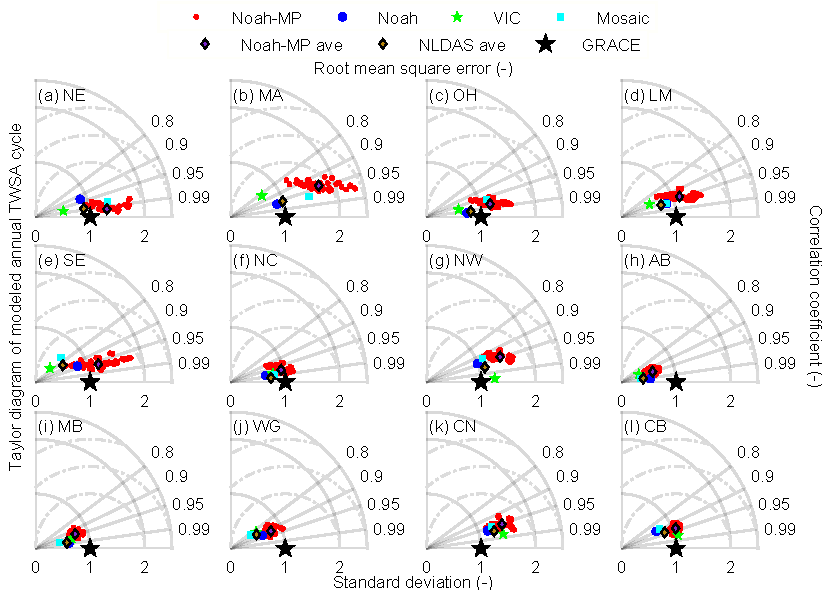
\includegraphics[width=12cm]{fig/fig02.pdf}
  \caption{Taylor diagram of TWSA's annual cycle for the 48 Noah-MP configurations (red dots) and three NLDAS models (blue dots for Noah, green stars for VIC, and cyan square for Mosaic) at the twelve RFCs. Black stars denote the observations. The ensemble mean of Noah-MP and NLDAS is presented by purple and dark golden diamonds, respectively. The distance between the model and observation presents the nuRMSE\@. The radial lines show the correlation coefficient, while the distance to the origin along the line denotes the normalized variability.}
  \label{fig:twsa:ancy:tss}
\end{figure*}

\begin{figure*}[t]
  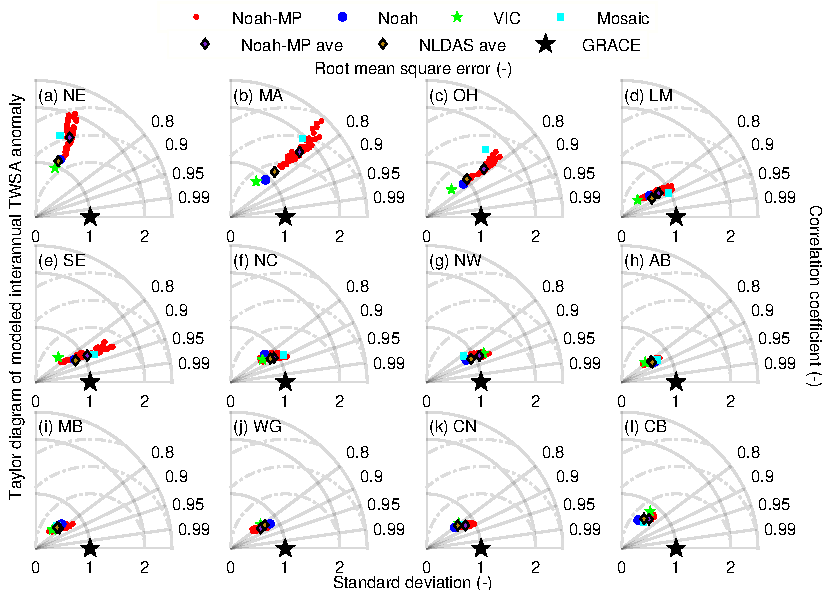
\includegraphics[width=12cm]{fig/fig03.pdf}
  \caption{As in Figure~\ref{fig:twsa:ancy:tss}, but for the interannual anomaly of TWSA.}
  \label{fig:twsa:anom:tss}
\end{figure*}

Figure~\ref{fig:twsa:ancy} shows the annual cycle of the TWSA estimated from GRACE, Noah-MP, and NLDAS\@. Figure~\ref{fig:twsa:ancy:tss} presents the TSS\@. In the 12 RFCs over CONUS, the TWSA peaks in spring, declines rapidly in summer, reaches a minimum in autumn, and recovers in winter. In terms of the timing of the peak and trough, Noah-MP and the NLDAS models perform similarly. In terms of the amplitude of variation, Noah-MP generally produces higher values in all RFCs. Previous studies have attributed this difference to the inclusion of a bucket groundwater component in Noah-MP \citep{cai2014JGRAa, ma2017JGRA}. However, we found the Noah-MP configurations without a groundwater component can still produce a higher amplitude, especially considering the structural similarity between Noah-MP and Noah. Further investigation of the model difference is necessary.

Figure~\ref{fig:twsa:ancy:tss} shows the Taylor diagram for the annual cycle of TWSA\@. The Noah-MP configurations generally outperform the NLDAS models in most of the RFCs, which results in the superior performance of the ensemble mean (shown in Table S5). Detailed examination of the TSS reveals that Noah-MP and NLDAS have similar correlation coefficients. Their difference is manifested in the modeled standard deviation (i.e., the amplitude of variation). In NE, MA, NW, and CN, Noah-MP underperforms compared with NLDAS, mainly due to overestimating the standard deviation. However, the interpretation of the overestimation is multifaceted. First, Noah-MP could overestimate the variability due to unsuitable parameters. For instance, specific yield is an important parameter for the simulation of groundwater storage and water level \citep{lv2021JAMES}. The parameter is calibrated as 0.2 by global simulations \citep{niu2007JGRa}. The globally calibrated value may be overestimated in the RFCs, leading to an overestimation in TWSA\@. Second, the GRACE data could underestimate the temporal variability at these coastal RFCs due to signal leakage from the ocean \citep{cai2014JGRAa}. In AB and MB, Noah-MP performs slightly better than the NLDAS models, but both underestimate the standard deviation. The Ogallala Aquifer encompasses the two RFCs. Noah-MP can better present the groundwater changes than the NLDAS models due to an unconfined aquifer module. But Noah-MP does not include the confined aquifers, leading to an underestimation of the groundwater storage variability.

Figure~\ref{fig:twsa:anom:tss} shows the Taylor diagram for the interannual anomaly of TWSA\@. Compared with the annual cycle (Figure~\ref{fig:twsa:ancy:tss}), both the Noah-MP configurations and the NLDAS models degrade significantly. Noah-MP still performs better than NLDAS in most RFCs. However, the superiority is marginal. In three RFCs---namely NE, MA, and OH, Noah-MP notably underperforms NLDAS\@. The underperformance is mainly due to higher variability than GRACE\@. Similar to the annual cycle, possible reasons include: (1) Noah-MP overestimated the variability due to unsuitable parameter values and (2) GRACE underestimated the variability due to the signal leaked from oceans.

\subsection{Soil moisture} \label{sec:results:sm}

\begin{figure*}[t]
  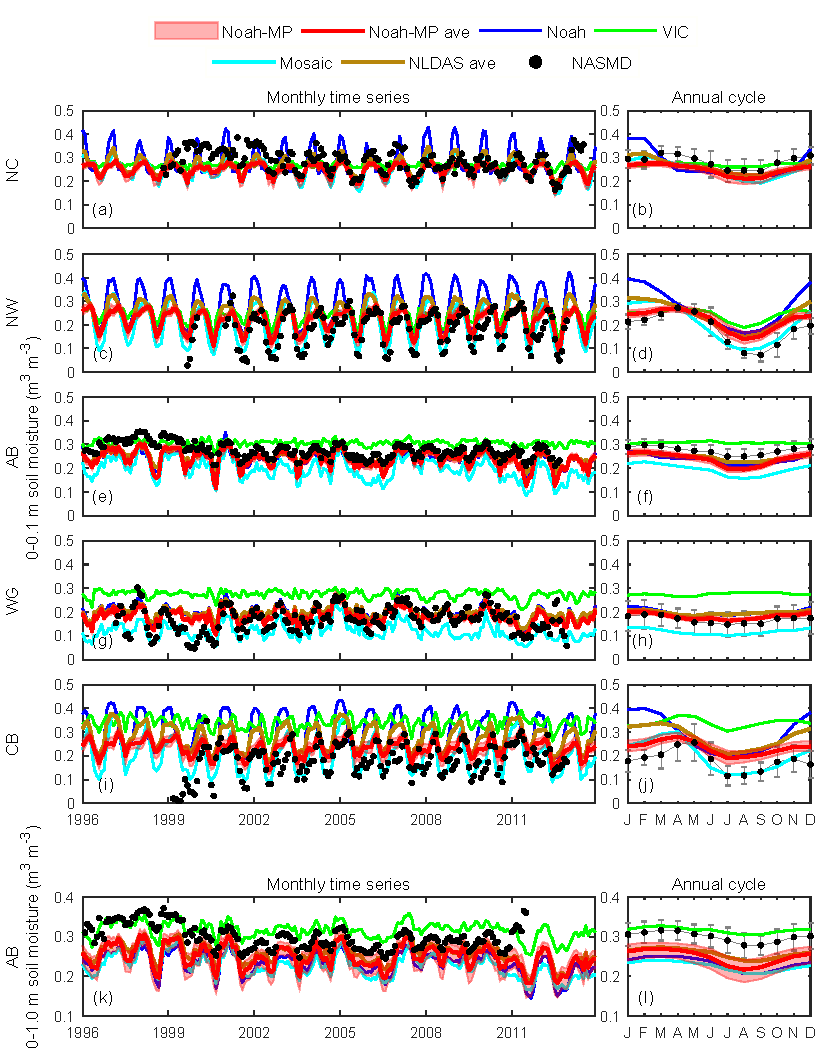
\includegraphics[width=12cm]{fig/fig04.pdf}
  \caption{Monthly surface (0--0.1\,m) and root-zone (0--1\,m) soil moisture (left column) and the annual cycle (right column) from the Noah-MP ensemble, the NLDAS models, and the NASMD observations for the period 1996--2013. Only the RFCs with more than ten observational sites are considered. Black dots denote the arithmetic average of the valid NASMD observations. Error bars in the right columns denote the standard deviation of the year-to-year differences. The shaded areas denote the range between the maxima and minima of the 48 Noah-MP estimates. The solid red line denotes the Noah-MP multi-physics ensemble mean. The three NLDAS models (Noah, Mosaic, VIC) and their ensemble mean are denoted by the blue, green, cyan, and dark golden lines, respectively. The five RFCs are sorted based on climatic aridity.}
  \label{fig:sm:ts}
\end{figure*}

\begin{figure*}[t]
  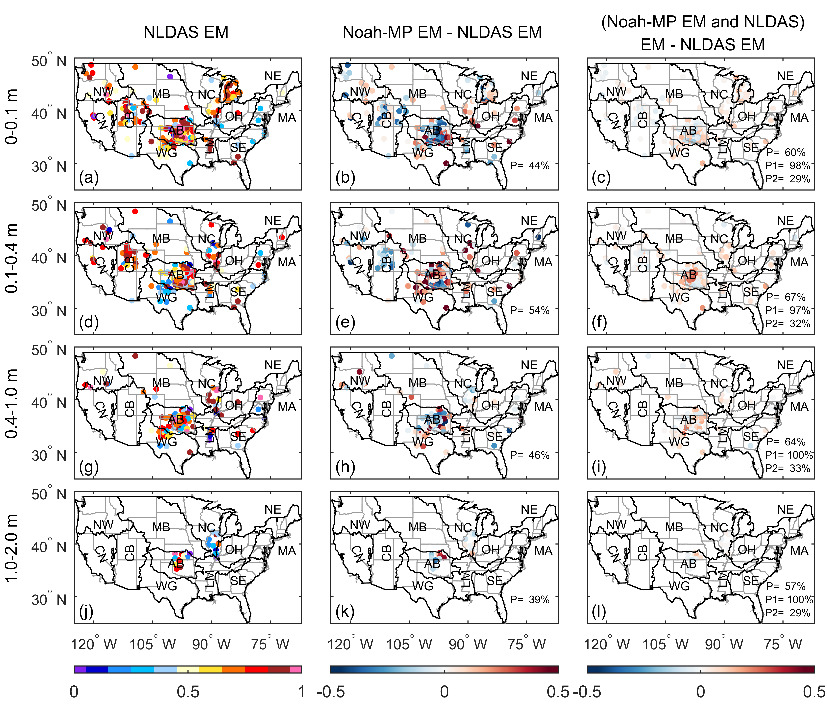
\includegraphics[width=12cm]{fig/fig05.pdf}
  \caption{The first column shows the TSS of the NLDAS ensemble mean in simulating the annual cycle of soil moisture at different depths (0--0.1\,m, 0.1--0.4\,m, 0.4--1\,m, 1--2\,m). The second column presents the difference in TSS between the Noah-MP ensemble mean and the NLDAS ensemble mean. The third column depicts the TSS difference between the arithmetic average of the Noah-MP ensemble mean and the NLDAS models to the NLDAS three-model mean. \(P\) is the percentage of sites at which a higher TSS appears relative to the NLDAS ensemble mean. \(P1\) (\(P2\)) is the percentage of sites at which a higher TSS appear given that the Noah-MP ensemble mean outperforms (underperforms) the NLDAS ensemble mean. The evaluation period is 1996--2013.}
  \label{fig:sm:ancy:tss}
\end{figure*}

\begin{figure*}[t]
  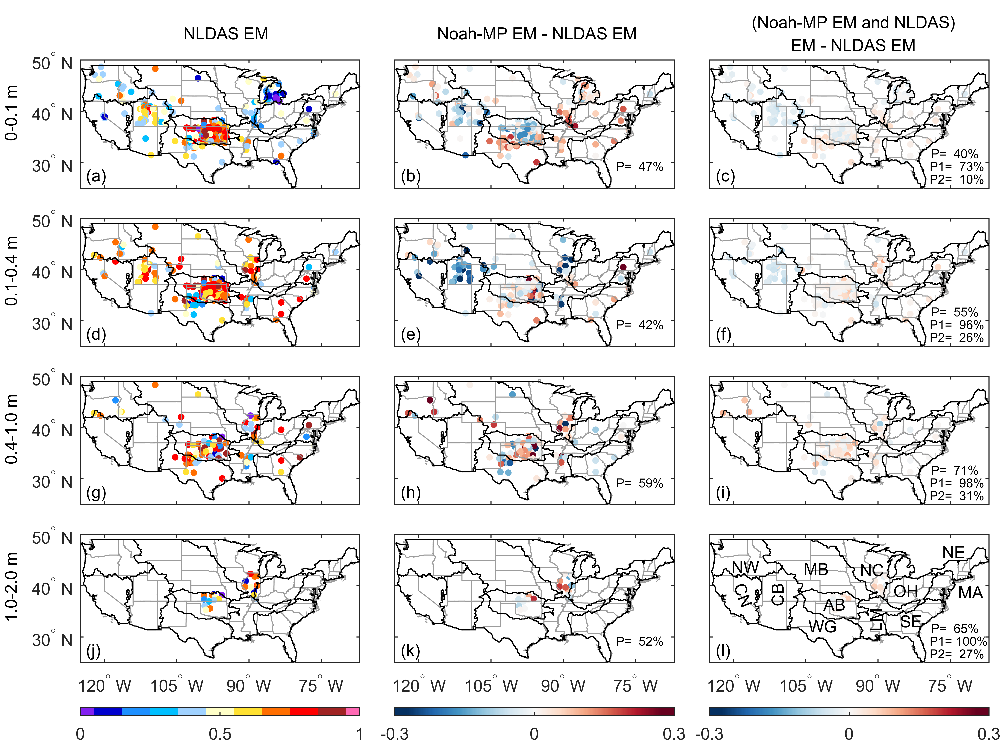
\includegraphics[width=12cm]{fig/fig06.pdf}
  \caption{As in Figure~\ref{fig:sm:ancy:tss}, but for interannual anomaly.}
  \label{fig:sm:anom:tss}
\end{figure*}

Figure~\ref{fig:sm:ts} presents the time series of the surface (0--0.1\,\unit{m}) and root-zone (0--1.0\,\unit{m}) soil moisture in NC, NW, AB, WG, and CB\@. These RFCs were selected as they have more than ten valid sites. Table S6 presents the corresponding TSSs. The Noah-MP configurations are consistent in estimating the surface soil moisture, having a spread remarkably smaller than that among the three NLDAS models. The NLDAS models have more diverse representations of soil moisture. Noah is the same as Noah-MP\@. Both solve Richards' equation to present the soil moisture dynamics in four layers \citep{niu2011JGRA}. Mosaic also solves Richards' equation but at three soil layers. The top layer is further divided into tiles to better represent spatial heterogeneity\citep{koster1992JGRA}. VIC is different from them, utilizing a conceptual soil water tank \citep{liang1994JGRA}. It could be that Noah-MP underestimated the ensemble spread, especially when considering its inability to represent the subgrid heterogeneity. The NLDAS models could also overestimate the spread when considering the conceptual representation of VIC\@. The spread among the Noah-MP configurations increases significantly from the surface (Figure~\ref{fig:sm:ts}e) to the root zone (Figure~\ref{fig:sm:ts}k). The ensemble spread in the root-zone soil moisture reflects the difference in modeling root-water uptake for plant transpiration and soil-bottom drainage as described in Appendix~\ref{sec:app:noahmp}. Further investigation (Figures S2--S5) shows that, in the deep layers (the third and fourth layers), Noah-MP has a comparable or greater spread than NLDAS\@.

Comparison between Noah-MP and Noah shows that they perform similarly in AB (Figures~\ref{fig:sm:ts}e and \ref{fig:sm:ts}f) and WG (Figures~\ref{fig:sm:ts}g and \ref{fig:sm:ts}h) but are different in NC (Figures~\ref{fig:sm:ts}a and \ref{fig:sm:ts}b), NW (Figures~\ref{fig:sm:ts}c and \ref{fig:sm:ts}d), and CB (Figures~\ref{fig:sm:ts}i and \ref{fig:sm:ts}j). The similarity in AB and WG is reasonable since the two models have similar soil layer structures and parameterizations. The dissimilarity in NC, NW, and CB is most pronounced in winter. It could result from the different snow parameterizations in Noah-MP and Noah, which is investigated in Section~\ref{sec:results:swe}.

In the RFCs and soil layers examined in Figure~\ref{fig:sm:ts}, the Noah-MP ensemble mean performs similarly or better than the NLDAS ensemble mean except in AB and CB\@. The superiority of the Noah-MP in simulating soil moisture is also reported in previous evaluations \citep{cai2014JGRAa}. In AB and CB, individual NLDAS models do not show a consistent superiority over Noah-MP\@. In AB, the best NLDAS model is VIC in winter and Noah in summer. The performance of VIC in winter corresponds to the best-performing snow estimation (Figure~\ref{fig:swe:ancy}h). In CB, the best NLDAS model is Noah in winter and Mosaic in summer. Mosaic carefully considers the subgrid variability of soil moisture, which could lead to better skill in RFCs with complex topography such as CB and NW\@. The NLDAS ensemble mean takes the advantage of wintertime soil moisture from VIC in AB and summertime soil moisture from Mosaic in CB\@. Both the advantage of VIC and Mosaic come from the representation of subgrid heterogeneity.

Figures~\ref{fig:sm:ancy:tss} and \ref{fig:sm:anom:tss} compare the TSS between the NLDAS and Noah-MP ensemble mean at each NAMSD site for the annual cycle and interannual anomaly, respectively. The comparison varies significantly with site and soil layer depth, revealing two major patterns. First, similar to Figure~\ref{fig:sm:ts}, NLDAS tends to outperform Noah-MP in AB and CB\@. The high skill of the NLDAS ensemble mean is likely a result of a high ensemble skill gain \citep{fei2021WRR} related to the diversity among the NLDAS models. Noah-MP has both a low ensemble spread and an inadequate representation of subgrid heterogeneity in the two RFCs. Second, Noah-MP outperforms NLDAS in other RFCs. In NC, OH, and MA, the low performance of NLDAS is related to the anomaly in winter-time soil moisture (Figure S2). The anomaly suggests that the NLDAS models generally have difficulty in modeling snow and snow-soil moisture interactions (refer to Section~\ref{sec:results:swe} for more information). On the other hand, Noah-MP has a better snow module, leading to a higher soil moisture estimation skill.

To maximize the utilization of the NLDAS model diversity and Noah-MP physics improvements, we combine the Noah-MP ensemble mean and the three NLDAS models. The right-hand columns of Figures~\ref{fig:sm:ancy:tss} and \ref{fig:sm:anom:tss} show that the four estimates' arithmetic average outperforms the three-model NLDAS ensemble mean at most NASMD sites. The outperformance suggests an added value of the Noah-MP data. If the Noah-MP ensemble mean already outperforms the NLDAS ensemble mean, the added value appears in almost every site. If the Noah-MP ensemble mean underperforms the NLDAS ensemble mean, the added value can still show up at approximately one-third (one-fourth) of the sites for the annual cycle (interannual anomaly).

\subsection{Snow water equivalent}\label{sec:results:swe}

\begin{figure}[t]
  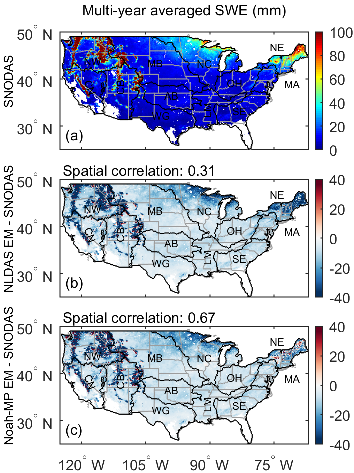
\includegraphics[width=8.3cm]{fig/fig07.pdf}
  \caption{(a) Spatial distribution of the 11-year-averaged (September 2004 to August 2015) SWE from SNODAS\@. (b) Difference between the NLDAS ensemble mean and SNODAS\@. (c) Difference between the Noah-MP ensemble mean and SNODAS\@. The spatial correlation coefficients between the NLDAS/Noah-MP ensemble mean and SNODAS are also presented.}
  \label{fig:swe:clim}
\end{figure}

\begin{figure*}[t]
  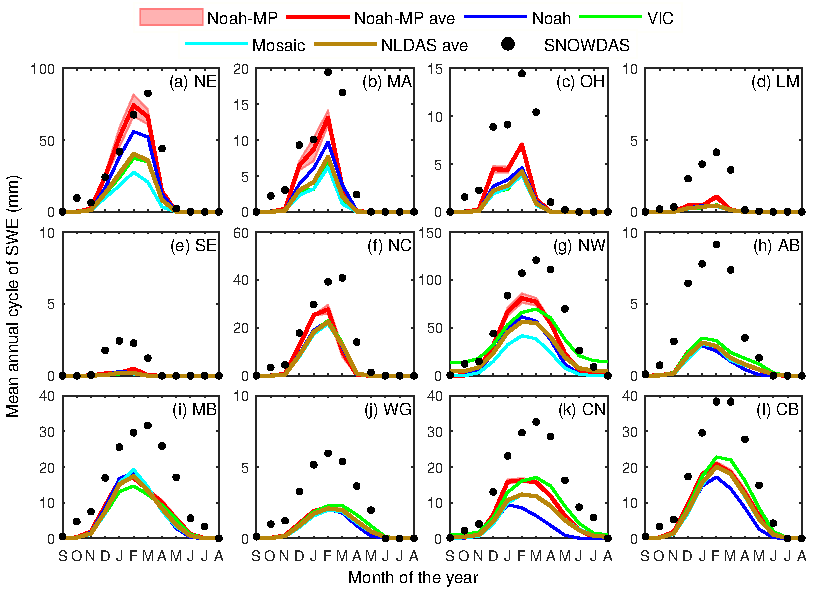
\includegraphics[width=12cm]{fig/fig08.pdf}
  \caption{As in Figure~\ref{fig:twsa:ancy}, but for SWE between September 2004 and August 2015.}
  \label{fig:swe:ancy}
\end{figure*}

\begin{figure*}[t]
  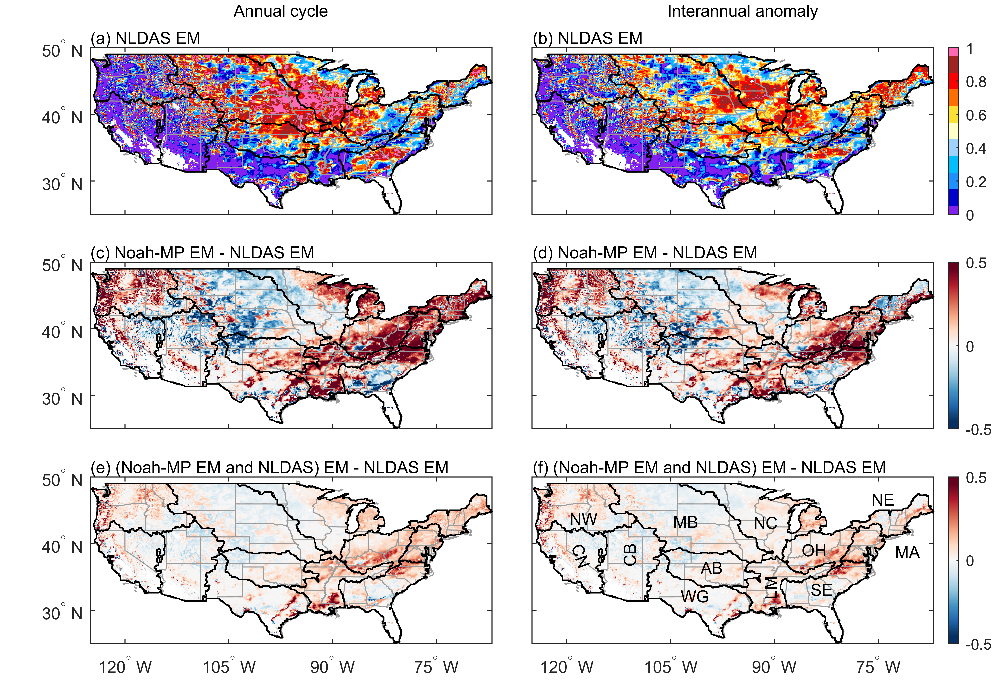
\includegraphics[width=12cm]{fig/fig09.pdf}
  \caption{TSS of the ensemble means in simulating the annual cycle (left column) and interannual anomaly (right column) of SWE\@. (a) and (b) TSS of the NLDAS ensemble mean. (c) and (d) the difference in TSS between the Noah-MP ensemble mean and the NLDAS ensemble mean. (e) and (f) the difference between the arithmetic average of the Noah-MP ensemble mean and three NLDAS models to the NLDAS ensemble mean. The evaluation period is 2004--2015.}
  \label{fig:swe:tss}
\end{figure*}

Figure~\ref{fig:swe:clim}a presents the spatial patterns of the multi-year-averaged SWE (\(W_{snow}\)) from SNODAS\@. Snow is mainly distributed in the northeast (NE, NC, OH, and MA) and in the mountains of the West (the Cascade Mountains, Rocky Mountains, Sierra Nevada in NW, AB, MB, WG, CN, and CB). Figure~\ref{fig:swe:clim}b (\ref{fig:swe:clim}c) shows the geographical difference between the Noah-MP (NLDAS) ensemble mean and SNODAS\@. Both Noah-MP and NLDAS exhibit a considerable underestimation in most areas of CONUS\@. However, the underestimation of Noah-MP is generally smaller. Figure~\ref{fig:swe:clim}d confirms that both Noah-MP and the NLDAS models tend to underestimate SWE in most areas but exhibit an overestimation when snow is extremely thick (SWE is greater than \qty{400}{mm}). Noah-MP performs better than the NLDAS models in most cases. The superiority of Noah-MP is likely attributable to the three-layer snowpack module, which can represent snow dynamics better in a wide range of snow depth than the single-layer Noah and Mosaic snow module and the quasi-two-layer VIC snow module. A careful consideration of the surface energy balance can also contribute to Noah-MP's superiority over VIC and Mosaic. Consequently, Noah-MP captures the spatial patterns better than NLDAS, with a spatial correlation of 0.87 versus 0.43. Further examination reveals that the superiority of Noah-MP appears in all elevation bands and is the most significant between 1000 to 2000\,m with a spatial correlation of 0.85 versus 0.38 (0.77 versus 0.76 below 1000\,m, and 0.89 versus 0.75 above 2000\,m).

Figure~\ref{fig:swe:ancy} compares the annual cycle estimated from SNODAS, NLDAS, and Noah-MP\@. The annual cycle in the twelve RFCs exhibits a similar pattern: it accumulates in winter, peaks in spring, and melts from late spring to summer. The snow season in the northeastern RFCs (i.e., NE, MA, OH, and NC) spans from October to May, whereas the snow season is longer in the mountainous RFCs of the West (i.e., NW, AB, MB, WG, CN, and CB), lasting to June. From the comparison between Noah-MP and NLDAS, we make three observations. First, consistent with Figure~\ref{fig:swe:clim}, the NLDAS models underestimate the SWE in all RFCs. Among the three NLDAS models, Noah performs the best in the northeast (e.g., NE, MA, and OH), whereas VIC shows some advantages in the western mountainous RFCs (e.g., NW, CN, and CB). Possible reasons for the Noah superiority in the northeast include the careful consideration of the surface energy balance, whereas, in the western mountains, the elevation bands of VIC can better capture the spatial heterogeneity. Second, Noah-MP outperforms the NLDAS models in almost all RFCs, except for showing a marginal degradation in AB and MB\@. In these two RFCs, VIC outperforms not only the NLDAS models but also Noah-MP\@. The terrain is hilly, and the elevation-banded parameterization enables a better representation of subgrid snow variability. Another reason is related to the shallow snow in these two RFCs. Noah-MP has known been experiencing negative biases with shallow snow (i.e., AB, MB, and WG). The bias is attributable to the shallow snow albedo as discussed in \citet{dang2019TC} and \citet{wang2020JHd}. Third, the ensemble spread among the Noah-MP configurations is small. The estimates of SWE and its uncertainty should be improved in the future by considering processes such as rain-snow partitioning \citet{wang2019GRL}, snow albedo \citep{wang2020JHd, dang2019TC}, roughness length \citep{he2019JGRA}.

Figure~\ref{fig:swe:tss} shows the TSS of the NLDAS and Noah-MP ensembles in estimating the annual cycle and interannual anomaly of SWE\@. Table S7 summarizes the skill scores for the twelve RFCs. The annual cycle and interannual anomaly exhibit similar spatial patterns. NLDAS performs well in most parts of the CONUS, with TSSs higher than 0.75. In MB, TSS reaches a minimum of 0.60. In comparison with NLDAS, Noah-MP performs notably better in the east and west but marginally worse in parts of the central CONUS\@. The location of Noah-MP's underperformance coincides well with shallow snow and relatively flat terrain. The coincidence hints at the weakness of Noah-MP in simulating shallow snow and the advantage of VIC in representing subgrid snow variability as discussed previously.

We further averaged the 48 Noah-MP configurations and added their average to the three-model NLDAS ensemble. Figures~\ref{fig:swe:tss}e and \ref{fig:swe:tss}f show that the four-estimate ensemble mean outperforms the three-model NLDAS ensemble mean in nearly all areas of CONUS, again proving the added value of the data provided in this paper.

\subsection{Evapotranspiration}\label{sec:results:et}

\begin{figure*}[t]
  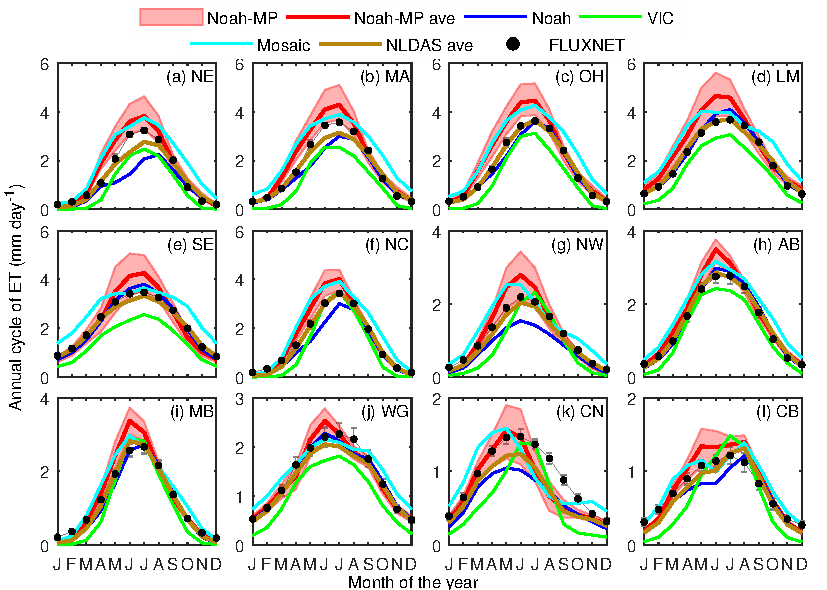
\includegraphics[width=12cm]{fig/fig10.pdf}
  \caption{As in Figure~\ref{fig:twsa:ancy}, but for ET in the period of 1982--2011.}
  \label{fig:et:ancy}
\end{figure*}

\begin{figure*}[t]
  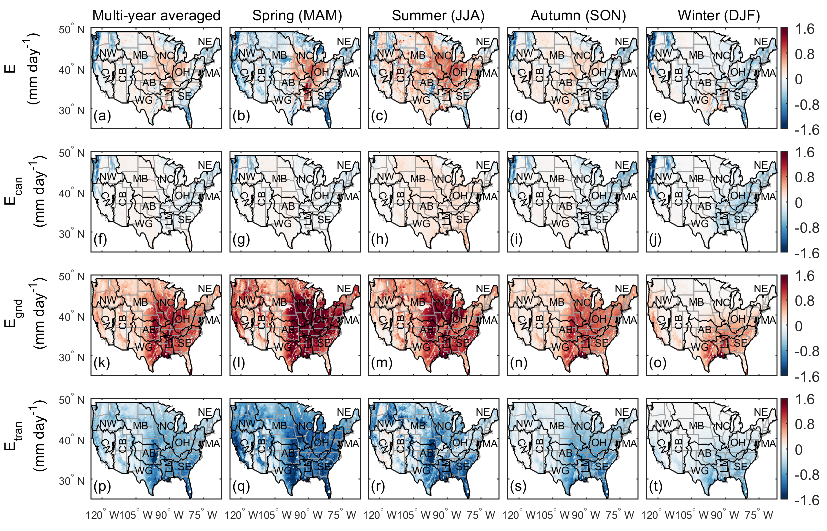
\includegraphics[width=12cm]{fig/fig11.pdf}
  \caption{Differences between the Noah-MP ensemble mean and GLEAM in total ET (\(E\)), canopy evaporation (\(E_{can}\)), ground evaporation (\(E_{gnd}\)), and transpiration (\(E_{tran}\)). The units are \unit{mm.day^{-1}}.}
  \label{fig:et:decomp}
\end{figure*}

\begin{figure}[t]
  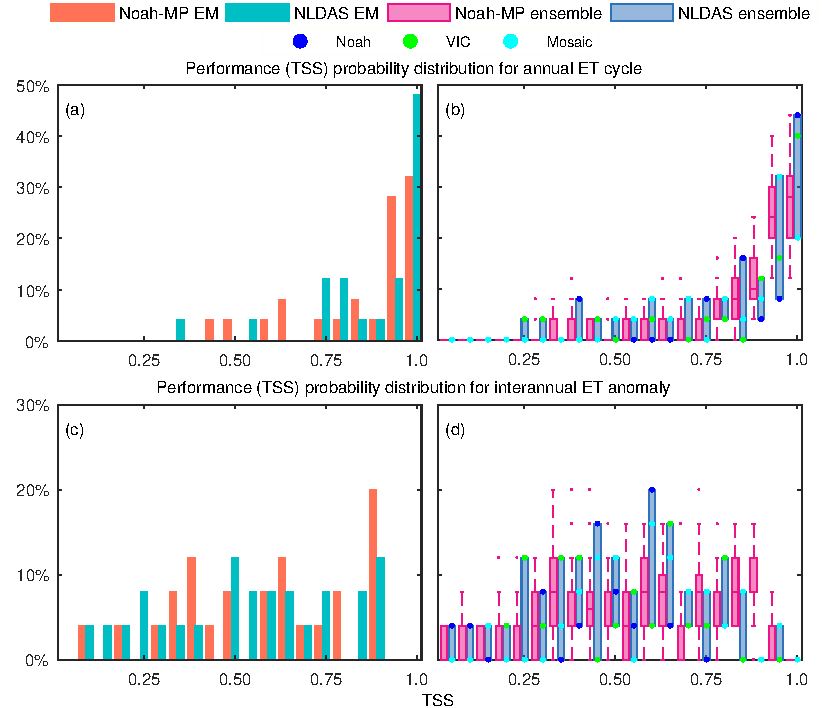
\includegraphics[width=8.3cm]{fig/fig12.pdf}
  \caption{Probability distribution of ET's TSS for the annual cycle (a, b) and interannual anomaly (c, d). The left column compares the Noah-MP (orange) and NLDAS (cyan) ensemble means. The right column reveals the Noah-MP (magenta) and NLDAS (dark blue) ensembles. The upper, middle, and lower quantile lines of the magenta boxes show the 75th, 50th, and 25th percentile values of the Noah-MP ensemble. The upper, middle, and lower lines of the dark blue boxes show the three NLDAS models. The blue, green, and cyan dots denote Noah, VIC, and Mosaic, respectively. The evaluation period can be found in Table S1.}
  \label{fig:et:tss}
\end{figure}

\begin{figure*}[t]
  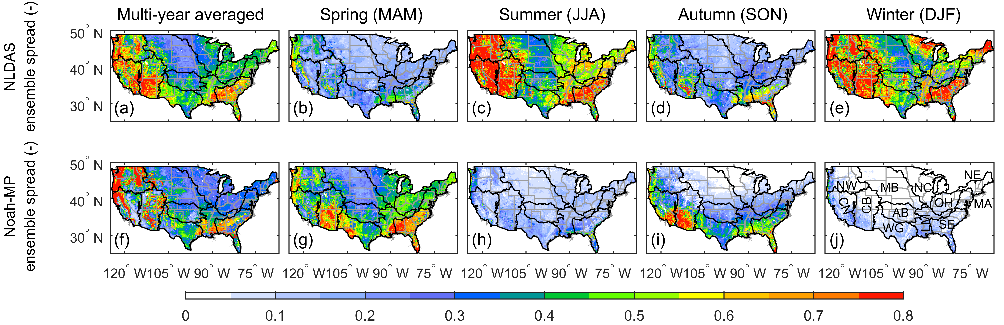
\includegraphics[width=12cm]{fig/fig13.pdf}
  \caption{Normalized ensemble spread of the multi-year averaged annual (first row) and seasonal (second--fifth rows) ET from NLDAS (first column) and Noah-MP (second column). The ensemble spread is normalized by the temporal variability of the FLUXNET MTE ET calculated using equation~\eqref{eq:var:total}.}
  \label{fig:et:spread}
\end{figure*}

\begin{figure*}[t]
  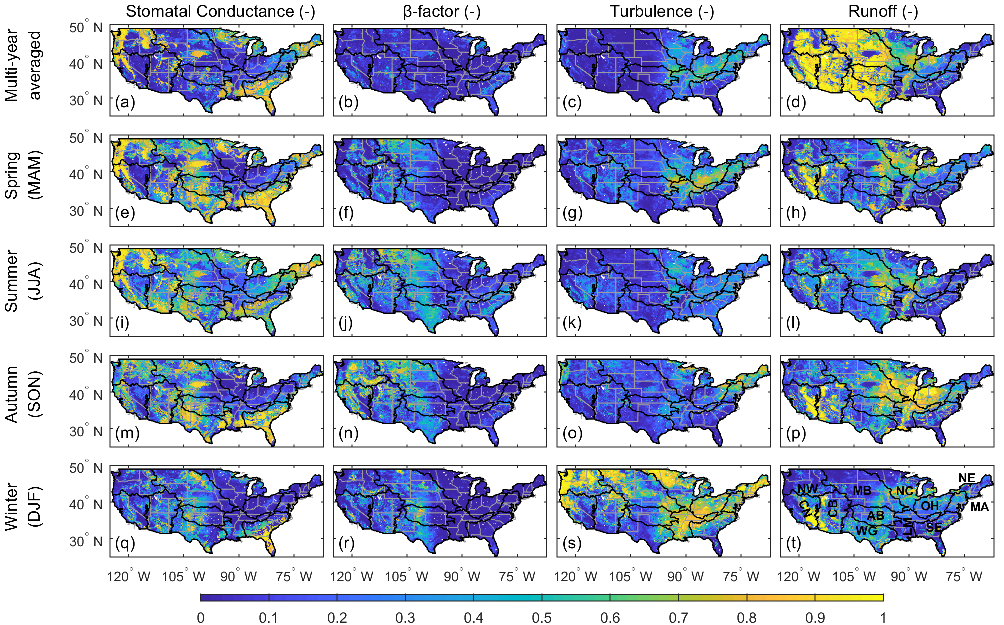
\includegraphics[width=12cm]{fig/fig14.pdf}
  \caption{The Sobol' total sensitivity of the multi-year-averaged and seasonal (spring---MAM, summer---JJA, autumn---SON, winter---DJF) ET to the four parameterizations: stomatal conductance, soil moisture limitation to transpiration (\beta{}-factor), turbulence, and runoff. Higher values indicate higher sensitivities.}
  \label{fig:et:sens}
\end{figure*}

Figure~\ref{fig:et:ancy} compares the annual cycle estimated from FLUXNET MTE, NLDAS, and Noah-MP in the twelve RFCs. We choose FLUXNET MTE as the reference here since its performance is superior when compared to AmeriFlux (Tables S2--S4). In all the twelve RFCs, ET peaks during summer and is lowest during winter. Noah-MP successfully captures the timing of the peak in humid RFCs (i.e., NE, MA, OH, LM, SE, NC, and NW) but shows a one-month lead in a few semi-arid and arid RFCs (i.e., MB, WG, and CN). The average of the three NLDAS models better reproduces the timing of the peak, but the models differ from each other significantly. Among the Noah-MP and NLDAS ensembles, VIC and Mosaic are notably different. VIC exhibits a systematic underestimation, while Mosaic shows an overall overestimation. The 48 Noah-MP configurations and Noah perform closely during autumn and winter, whereas their differences are pronounced during spring and summer. During spring and summer, Noah is the closest to FLUXNET MTE in most RFCs except NE and MA, whereas Noah-MP constantly overestimates the ET in all RFCs.

The overestimation of Noah-MP was investigated by separately comparing the three components of ET (i.e., transpiration, canopy evaporation, and ground evaporation) with GLEAM (Figure S6). Figure~\ref{fig:et:decomp} shows the overestimation of total ET is closely linked to the overestimation of ground evaporation, which could be partially attributable to the overly high roughness length for heat and water, as described in Appendix~\ref{sec:app:noahmp:chen97} and \ref{sec:app:noahmp:mo}. Besides, the lack of a litter layer \citep{decker2017JAMES} in Noah-MP could also play a part.

Figure~\ref{fig:et:tss} evaluates Noah-MP and NLDAS using the 25 AmeriFlux sites. The NLDAS ensemble mean outperforms the Noah-MP ensemble mean for the annual cycle, and this outperformance results from two causes. First, an NLDAS member, Noah, performs the closest to the observations, as shown in Figures \ref{fig:et:tss}b and \ref{fig:et:ancy}. Second, the three NLDAS models are remarkably different from each other. The diversity of the ensemble gives a higher skill gain by combining them, as shown by the difference between the ensemble mean skill (Figures \ref{fig:et:tss}a) and the median TSS (Figures~\ref{fig:et:tss}b). On the other hand, the Noah-MP configurations are too similar to each other, and all have a positive bias (Figure~\ref{fig:et:ancy}). However, for the interannual anomaly, the Noah-MP ensemble mean slightly outperforms the NLDAS ensemble mean (Figure~\ref{fig:et:tss}c). Figure~\ref{fig:et:tss}d shows that the Noah-MP configurations marginally outperform the NLDAS models. Among the NLDAS models, VIC performs the best, and Noah does not exhibit the same superiority shown in the annual cycle. The difference between the NLDAS ensemble mean performance (Figure~\ref{fig:et:tss}c) and median performance (Figure~\ref{fig:et:tss}d) is marginal, suggesting that the NLDAS ensemble skill gains are not notable for the interannual anomaly.

Figure~\ref{fig:et:spread} examines the ensemble spread of Noah-MP and NLDAS\@. The ensemble spread is normalized by the temporal variability calculated using the FLUXNET MTE ET\@. NLDAS has a significant spread in the southeast and west in all seasons, while spring shows the largest value. As seen in Figure~\ref{fig:et:ancy}, the NLDAS ensemble spread mainly reflects the differences between VIC and Mosaic. The Noah-MP ensemble has a notably smaller spread than NLDAS\@. The Noah-MP ensemble spread is manifested in spring and summer in the southeastern (SE, LM, and WG) and western (CN, CB, and NW) RFCs.

We can decompose the Noah-MP ensemble spread and pinpoint the dominant process using Sobol' sensitivity analysis \citep{zheng2019WRR}. Figure~\ref{fig:et:sens} delineates the Sobol' total sensitivity index of total ET to the four processes described in Appendix~\ref{sec:app:noahmp}. In spring and summer, for the regions where the Noah-MP configurations show significant spread (SE, LM, WG, CB, CN, and NW) (Figure~\ref{fig:et:spread}), ET is most sensitive to the parameterization of stomatal conductance (Figures~\ref{fig:et:sens}e and \ref{fig:et:sens}i) and then to the \beta{}-factor (Figures~\ref{fig:et:sens}f and \ref{fig:et:sens}j). However, for regions with positive biases (NC, OH, and LM, as shown in Figures~\ref{fig:et:decomp}b and \ref{fig:et:decomp}c), the Noah-MP estimation is more sensitive to the turbulence parameterizations (Figures~\ref{fig:et:sens}c and \ref{fig:et:sens}g). During autumn and winter, the parameterizations of stomatal conductance (Figures~\ref{fig:et:sens}m and \ref{fig:et:sens}q) and \beta{}-factor (Figures~\ref{fig:et:sens}n and \ref{fig:et:sens}r) still have significant impacts on the estimation of ET, and these impacts could be a result of the ``memory'' of TWS \citep{zheng2019WRR}. Besides these two processes, the runoff parameterization is dominant during autumn in the east (Figure~\ref{fig:et:sens}p), and the turbulence parameterization is dominant during winter (Figure~\ref{fig:et:sens}s).

\codedataavailability{
The dataset is freely available for download from the Zenodo online repository at \url{https://doi.org/10.5281/zenodo.7109816} (Zheng et al., 2022). The dataset (along with datasets on which it is based) is subject to a Creative Commons BY (attribution) license agreement (\url{https://creativecommons.org/licenses}, last access: 2021-08-16).
}\label{sec:availability}

\conclusions{}\label{sec:conclusions}

This paper describes a 1/8\degree{} dataset of the TWB over the CONUS from 1980 to 2015 simulated from an ensemble of 48 perturbed-physics configurations of Noah-MP\@. This Noah-MP multi-physics ensemble features an enrichment of the NLDAS-2 four-model ensemble and brings convenience for multi-model comparison. The dataset has already been used in the monitoring of groundwater storage change \citep{rateb2020WRR}, the analysis of LSM parameterization sensitivity \citep{zheng2019WRR}, the development of model evaluation method \citep{zheng2020JAMES}, and hydrological ensemble simulations \citep{fei2021WRR}. This paper details the Noah-MP parameterizations employed and evaluates the estimated TWSA, soil moisture, SWE, and ET in comparison with the NLDAS ensemble.

The spread of the ensemble estimation is the largest for the runoff. The spread in surface runoff accounts for 34\% of its climatological mean. The spread is comparable to the previous estimates for multi-model ensembles \citep{dirmeyer2006BAMS}. The ensemble spread in snow water equivalent is the smallest, 2.5\% of its climatological mean. The ensemble has not included different parameterizations of several snow processes such as rain-snow partitioning, snow albedo, and roughness length, which could lead to an underestimation of the ensemble spread. The underestimation of the ensemble spread becomes more apparent when the Noah-MP ensemble mean is biased (Figure~\ref{fig:swe:ancy}). The bias is more pronounced relative to the NLDAS models in parts of AB and MB where snow is shallow and the terrain is hilly (Figure~\ref{fig:swe:tss}). VIC performs better there, suggesting the importance of considering subgrid variability.

Evaluation against various reference data shows that Noah-MP generally performs better than the NLDAS models. The augmented three-layer snow module of Noah-MP significantly improves the estimation of snow and also wintertime soil moisture. On the other hand, the NLDAS models outperform Noah-MP in AB and CB for surface soil moisture (Figures~\ref{fig:sm:ts} to \ref{fig:sm:anom:tss}), in AB and MB for snow (Figures~\ref{fig:swe:ancy} and \ref{fig:swe:tss}), and in OH, LM, and NC for the annual cycle of ET (Figure~\ref{fig:et:ancy}). The outperformance of NLDAS is likely attributable to the consideration of subgrid variability in soil moisture with Mosaic and in snow with VIC\@. The Noah-MP ensemble could be improved by increasing the spatial resolution or developing parameterizations of subgrid heterogeneity. Noah-MP also underestimates the temporal variability of TWS in coastal RFCs (Figures~\ref{fig:twsa:ancy:tss} and \ref{fig:twsa:anom:tss}). Correction of the ocean signal leakage in the GRACE data and representation of spatially varying parameter unconfined aquifer should be beneficial. For the annual cycle of ET, there is a systematic overestimation in spring and summer. Sobol' sensitivity analysis of the Noah-MP ensemble reveals that the bias is mainly related to the parameterization of turbulence. We have examined the code and found that the implementation is inconsistent with the literature. The parameterization of the roughness length of heat and water vapor likely contributes to the ET overestimation.

The Noah-MP ensemble shares the same atmospheric forcing and static parameters with the NLDAS models. The similarity enables the comparison between the multi-model and perturbed-physics ensembling methods as shown in \citet{fei2021WRR}. Besides, Noah-MP complements the NLDAS models well. Adding Noah-MP to the NLDAS ensemble can consistently improve the TWB variables in most areas of CONUS\@.

The Noah-MP model has been undergoing rapid development. New components such as plant hydraulics \citep{li2021JAMESa}, roughness sublayer \citep{abolafia-rosenzweig2021JAMES}, crops \citep{liu2016JGRA}, and dynamic rooting depth \citep{liu2020JAMES} have been added. New schemes for the processes such as rain-snow partitioning \citep{wang2019GRL} have been included. Parameterizations of surface roughness length \citep{he2019JGRA, zhang2021IJC}, snow albedo \citep{wang2020JHd}, and vertical soil layers \citep{zhao2022ITGRS,shellito2020JH} have been refined. The dataset can be improved by using the updated model and including more perturbations.

\appendix

\section{Formulation of the used noah-mp parameterization schemes}\label{sec:app:noahmp}

\subsection{SIMGM runoff parameterization scheme}\label{sec:app:noahmp:simgm}

SIMGM is a TOPMODEL-based runoff model \citep{niu2007JGRa}. The scheme parameterizes runoff (\(R_{srf}\) and \(R_{sub}\)) as an exponential function of groundwater table depth (\(z_{wt}\), \unit{m}, positive down) as follows.
\begin{equation}
  R_{srf} = Q_{soil,srf} [(1 - f_{frz,1}) f_{sat} + f_{frz,1} ]
  \text{,} \label{eq:simgm:rsrf}
\end{equation}
\begin{equation}
  f_{sat} = f_{sat,max} \exp[-0.5 f (z_{wt} - z_{bot})]
  \text{,} \label{eq:simgm:fsat}
\end{equation}
\begin{equation}
  R_{sub} = [1 - \max_{i=1,\dots,N_{soil}} (f_{frz,i})] R_{sub,max}
  \exp[-\Lambda - f(z_{wt} - z_{bot})]
  \text{,} \label{eq:simgm:rsub}
\end{equation}
where \(Q_{soil,srf}\) is the water incident on the soil surface (the sum of precipitation throughfall, snowmelt, and dewfall; \unit{kg.m^{-2}.s^{-1}}), \(f_{frz,i}\) is the fractional frozen area of the \(i\)-th soil layer (\unit{m^2.m^{-2}}), which is parameterized using the frozen water content of the soil layer following \citet{niu2006JH}, \(f_{sat}\) is the saturation fraction of the grid cell (\unit{m^2.m^{-2}}), and \(z_{bot}\) is the depth of the soil column bottom (2 m in this study), and \(z_{wt}\) is the groundwater table depth (m), which is converted from the groundwater storage by a specific-yield parameter. The groundwater storage is predicted using a dynamic groundwater model interacting with the soil column bottom \citep{niu2007JGRa}.

The scheme has four calibratable parameters: (1) \(f_{sat,max}\), the maximum saturation area fraction (\unit{m^2.m^{-2}}), which is defined as the cumulative distribution function of the topographic index when the grid-cell-mean water table depth is zero; (2) \(f\), a runoff decay factor (unitless); (3) \(R_{sub,max}\), the maximum subsurface runoff when the grid-cell-mean water table depth is zero (\unit{kg.m^{-2}.s^{-1}}); and (4) \(\Lambda\), the grid-cell-mean topographic index (unitless). In this study, the parameters have the following values: \(f_{sat,max} = 0.38\)\,\unit{m^2.m^{-2}}, $f=6$, $R_{sub,max}=5$\,\unit{kg.m^{-2}.s^{-1}}, and \(\Lambda = 10.5\).

\subsection{SIMTOP runoff parameterization scheme}\label{sec:app:noahmp:simtop}

SIMTOP is also a TOPMODEL-based runoff parameterization scheme, the same as SIMGM (equations~\eqref{eq:simgm:rsrf}--\eqref{eq:simgm:rsub}). The major difference between SIMTOP and SIMGM is that SIMTOP parameterizes the groundwater table depth (\(z_{wt}\)) using the soil liquid water content by assuming the water head is at equilibrium throughout the soil column down to the water table \citep{niu2005JGRA}. Although SIMTOP and SIMGM share the same conceptual model of runoff generation, implementation differences exist. First, in contrast to equations \eqref{eq:simgm:fsat} and \eqref{eq:simgm:rsub}, SIMTOP does not use the soil column bottom depth (\(z_{bot}\)) in calculating the saturation area fraction (\(f_{sat}\)) and subsurface runoff:
\begin{align}
  f_{sat} = & f_{sat,max} \exp(-0.5 f z_{wt})
  \text{,} \\
  R_{sub} = & [1-\max_{i=1,\cdots,N_{soil}}(f_{frz,i})]
  R_{sub,max} \exp(-\Lambda - f z_{wt})
  \text{.}
\end{align}
Second, parameter values are slightly different for the runoff decay factor and maximum subsurface runoff: \(f=2\), and \(R_{sub,max}=4\)\,\unit{kg.m^{-2}.s^{-1}}.

\subsection{NOAHR runoff parameterization scheme}\label{sec:app:noahmp:noahr}

NOAHR parameterizes surface runoff (\(R_{srf}\)) as infiltration excess:
\begin{equation}
  R_{srf} = Q_{soil,srf} - Q_{soil,in}
  \text{,}
\end{equation}
where \(Q_{soil,i}\) is the infiltration into the soil (\unit{kg.m^{-2}.s^{-1}}). The infiltration is derived from the approximate solution to the Richards equation following \citet{philip1969AiH} with additional considerations of the spatial variability of precipitation and infiltration capacity. By assuming exponential and independent distributions of precipitation and infiltration capacity within a model grid cell, NOAHR formulates the soil infiltration as follows:
\begin{align}
  Q_{soil,in} = & Q_{soil,srf} \frac{I_c}{Q_{soil,srf} \Delta t + I_c}
  \text{,} \\
  I_{c} =       & w_d [1-\exp(-K_{\Delta t} \Delta t)]
  \text{,} \\
  w_d =         & \sum_{i=1}^{N_{soil}} \rho_{wat} (w_{sat,i} - w_{soil,i}) \Delta z_{soil,i}
  \text{,}
\end{align}
where \(I_{c}\) is the soil infiltration capacity of the model grid cell (\unit{kg.m^{-2}}), \(w_d\) is the water deficit of the soil column (\unit{kg.m^{-2}}), and \(\Delta t\) is the model time step (s). Following \citep{chen2001MWR}, the parameter is assumed as propositional to the saturated hydraulic conductivity of the first soil layer (\(K_{sat,1}\), \unit{kg.m^{-2}.s^{-1}}):
\begin{equation}
  K_{\Delta t} = \frac{K_{\Delta t,ref}}{k_{ref}} K_{sat,1}
  \text{,}
\end{equation}
where \(K_{\Delta t,ref}\) and \(k_{ref}\) are two parameters. In Noah-MP (and Noah), \(K_{\Delta t,ref} = \frac{3}{86400}\,\unit{s^{-1}}\), and \(k_{ref}=\qty{2e-3}{kg.m^{-2}.s^{-1}}\). \(K_{sat,1}\) is assigned using a soil parameter lookup table according to the soil texture type.

NOAHR assumes free drainage at the soil column bottom. The subsurface runoff is calculated as
\begin{equation}
  R_{sub} = \alpha_{slope} K_{soil,N_{soil}} \label{eq:noahr:rsub}
  \text{,}
\end{equation}
where \(\alpha_{slope}\) is the terrain slope index, which is arbitrarily given as 0.1 in the adopted version of Noah-MP\@. \(K_{soil,N_{soil}}\) is the hydraulic conductivity of the bottom soil layer, which is parameterized following \citet{clapp1978WRR}.

\subsection{BATS runoff parameterization scheme}\label{sec:app:noahmp:bats}

The BATS scheme parameterizes surface runoff (\(R_{srf}\)) as a funciton of soil wetness \citep{yang1996GPC}:
\begin{align}
  R_{srf} = & Q_{soil,srf} \left[ (1 - f_{frz,1}) f_{sat} + f_{frz,1} \right]
  \text{,} \\
  f_{sat} = & \theta^4
  \text{,} \\
  \theta =  & \frac{\sum_{i=1}^{N_{soil}}\frac{w_{soil,i}}{w_{sat,i}}\Delta
  z_{soil,i}}
  {\sum_{i=1}^{N_{soil}}\Delta z_{soil,i}}
  \text{,}
\end{align}
where \(\theta\) is the averaged wetness throughout the soil column (\unit{m^3.m^{-3}}).

Similar to NOAHR, the BATS scheme also assumes a free drainage boundary condition at the soil column bottom. Subsurface runoff (\(R_{sub}\)) is parameterized as follows:
\begin{equation}
  R_{sub} = \left(1 - \max_{i=1,\cdots,N_{soil}}(f_{frz,i})\right) K_{soil,N_{soil}}
  \text{.}
\end{equation}

\subsection{Ball--Berry scheme of stomatal resistance}\label{sec:app:noahmp:ballberry}

Leaf stomata are the small pores typically found on the underside of leaves. They control the gas exchange of CO\textsubscript{2}, H\textsubscript{2}O, and O\textsubscript{2} between the internal leaf structure and the external atmosphere. In LSMs, the opening and closing of the stomata are characterized by stomatal conductance.

The Ball--Berry scheme for parameterizing the stomatal conductance (\(g_{s}\)) for H\textsubscript{2}O is as follows:
\begin{equation}
  g_{s}   = m \frac{A}{c_{s}} \frac{e_{s}}{e_{i}} P_{atm} + b
  \text{,}
\end{equation}
where \(g_{s}\) is the leaf stomatal conductance (\unit{\mu mol.m^{-2}.s^{-1}}), \(m\) is a vegetation-type dependent parameter (unitless), \(A\) is the leaf photosynthesis rate, \(c_{s}\) is the CO\textsubscript{2} partial pressure at the leaf surface (\unit{Pa}), \(e_{s}\) is the water vapor pressure at the leaf surface (\unit{Pa}), \(e_{i}\) is the saturated water vapor at the stomata (\unit{Pa}), \(P_{atm}\) is the ambient air pressure (\unit{Pa}), and \(b\) is the stomatal conductance at zero photosynthesis (\unit{\mu mol.m^{-2}.s^{-1}}). The parameters \(m\) and \(b\) are assigned from a lookup table using the vegetation type.

\subsection{Jarvis scheme of stomatal resistance}\label{sec:app:noahmp:jarvis}

The Jarvis scheme for parameterizing the canopy resistance (\(R_{c}\)) based on the product of four stress factors (\unit{s.m^{-1}}) is calculated as follows \citep{chen1996JGRA, sellers1996JCa, jacquemin1990BM, jarvis1976PTRSLB}:
\begin{align}
  R_c =   & R_{c,min} \frac{1}{f_{1} f_{2} f_{3} \beta}
  \text{,} \\
  f_{1} = & \frac{\frac{R_{c,min}}{R_{c,max}}+f}{1+f}
  \text{,} \\
  f =     & 0.55 \frac{2 R_{g}}{R_{gl}}
  \text{,} \\
  f_{2} = & \frac{1}{1+h_s[q_{sat}(T_{l})-q_{a}]}
  \text{,} \\
  f_{3} = & 1- 0.0016 (T_{ref} - T_l)^2
  \text{,}
\end{align}
where \(f_{1}\), \(f_{2}\) and \(f_{3}\) are the stress factors of solar radiation, vapor pressure deficit, and air temperature, respectively (unitless), which are unitless and range from 0 to 1; \(\beta\) is the soil moisture stress factor, which is detailed in Section~\ref{sec:app:noahmp:beta}; \(R_{g}\) is the incoming solar radiation (\unit{W.m^{-2}}) for unit leaf area index; \(T_{l}\) is leaf temperature (\unit{K}). \(q_{sat}(T_l)\) (\unit{kg.kg^{-1}}) and \(q_a\) are the saturated humidity at the temperature of \(T_{l}\) (\unit{kg.kg^{-1}}) and ambient humidity, respectively. In literature \citep{chen1996JGRA, jacquemin1990BM}, \(q_{sat}{T_l}\) and \(q_a\) are specific humidity, whereas in Noah-MP v3.6, they are implemented as mixing ratio.

The scheme has five parameters: \(R_{c,min}\) the minimum stomatal resistance (\unit{s.m^{-1}}) per unit leaf area index; \(R_{c,max}\) the maximum resistance; \(R_{gl}\) a radiation scaling factor (unitless); \(h_{s}\) a humidity scaling factor (unitless); \(T_{ref}\) the optimum temperature (\unit{K}). Among these parameters, \(R_{c,min}\), \(R_{gl}\), and \(h_{s}\) are assigned using a vegetation-parameter lookup table, while \(R_{c,max}\) and \(T_{ref}\) are preassembly-assigned to \qty{5000}{s.m^{-1}} and \qty{298}{K}, respectively.

\subsection{Three soil moisture stress factor schemes}\label{sec:app:noahmp:beta}

The NOAHB scheme parameterizes the soil moisture stress factor controlling transpiration (\beta{}-factor) as a function of soil moisture, which is calculated as follows:
\begin{equation}
  \beta = \sum_{i=1}^{N_{root}} \frac{\Delta z_{soil,i}}{z_{root}}
  \min(1, \frac{\theta_i - \theta_{wilt}}{\theta_{ref} - \theta_{wilt}})
  \text{,}
\end{equation}
where \(N_{root}\) is the total number of soil layers that contain roots, \(z_{root}\) is the total depth of the root zone layer (\unit{m}), and \(\theta_i\) is the volumetric soil moisture of the \(i\)-th soil layer (\unit{m^3.m^{-3}}). NOAHB has two parameters: \(\theta_{ref}\) the field capacity (\unit{m^3.m^{-3}}); and \(\theta_{wilt}\), the wilting volumetric soil moisture (\unit{m^3.m^{-3}}).

The CLM scheme \citep{oleson2004} parameterizes \(\beta\) as a function of soil matric potential, which is calculated as follows:
\begin{equation}
  \beta = \sum_{i=1}^{N_{root}} \frac{\Delta z_{soil,i}}{z_{root}}
  \min(1, \frac{\psi_{wilt} - \psi_i}{\psi_{wilt} - \psi_{sat}})
  \text{,}
\end{equation}
where \(\psi_i\) is the water pressure head of the \(i\)-th soil layer (\unit{m}), and \(\psi_i\) is converted from \(\theta_i\) using the formula of \citet{clapp1978WRR}. CLM has two parameters: \(\psi_{sat}\), the saturated water pressure head (\unit{m}), and \(\psi_{wilt}\), the wilting pressure head (\unit{m}).

The SSiB scheme \citet{xue1991JC} also parameterizes the \beta{}-factor as a function of the soil pressure head, similar to CLM\@. However, the formula is different, as follows:
\begin{equation}
  \beta = \sum_{i=1}^{N_{root}} \frac{\Delta z_{soil,i}}{z_{root}}
  \min\left[1, 1 - \exp\left(-c_2 \ln(\frac{\psi_{wilt}}{\psi_{i}})\right)\right]
  \text{,}
\end{equation}
SSiB has two parameters: \(\psi_{wilt}\), the wilting pressure head (\unit{m}); and \(c_2\), a unitless coefficient.

In Noah-MP version 3.6, the parameters \(\theta_{sat}\), \(\theta_{wilt}\), and \(\psi_{sat}\) are assigned using a soil parameter lookup table \citep[Table 2]{chen2001MWR}; \(\psi_{wilt}\) is \qty{-10}{m}, independent of vegetation and soil types \citep{niu2011JGRA}; \(c_2\) is assumed constant at \num{5.8}, whereas in SSiB, this parameter varies with vegetation type \citep[Table 2]{xue1991JC}.

\subsection{Chen97 near-surface turbulence scheme}\label{sec:app:noahmp:chen97}

The Chen97 scheme \citep{chen1997BM} parameterizes the surface exchange coefficient for heat (\(C_{h}\)) as follows:
\begin{equation}
  C_{h} = \kappa^{2} \left[ \ln(\frac{z}{z_{0m}})
    - \Psi_{m}(\frac{z}{L})
    + \Psi_{m}(\frac{z_{0m}}{L})\right]^{-1}
  \left[\ln(\frac{z}{z_{0h}})
    - \Psi_{h}(\frac{z}{L})
    + \Psi_{h}(\frac{z_{0h}}{L})\right]^{-1}
  \text{,}
\end{equation}
where \(\kappa=0.4\) is the von Kármán constant; \(L\) is the Monin--Obukhov (M--O) length (m); \(z\) is the reference height (m); \(\Psi_{m}\) and \(\Psi_{h}\) are the similarity theory-based stability functions for momentum and heat, respectively; \(z_{0m}\) the roughness length for momentum (m), depends on the land cover/land-use type; and \(z_{0h}\) is the roughness length for heat (m). \citet{niu2011JGRA} parameterized \(z_{0h} = z_{0m} \exp(-\kappa C \sqrt{{Re}^*})\), where \(C=0.1\) and \({Re}^*\) is the roughness Reynolds number. However, in the code of Noah-MP version 3.6, \(z_{0h} = z_{0m}\).

\subsection{M--O near-surface turbulence scheme}\label{sec:app:noahmp:mo}

The M--O scheme is based on the M--O similarity theory \citep{brutsaert1982}, which parameterizes \(C_h\) as follows:
\begin{equation}
  C_h = \kappa^2 \left[ \ln(\frac{z - d_{0}}{z_{0m}})
    - \Psi_{m}(\frac{z - d_0}{L})\right]^{-1}
  \left[\ln(\frac{z - d_0}{z_{0h}})
    -\Psi_{h}(\frac{z - d_0}{L})\right]^{-1}
\end{equation}
where \(z_{0h} = z_{0m}\), and \(d_0\) is the zero-displacement height (m),
\begin{equation}
  d_0 = 0.64 z_{ct}
  \text{,}
\end{equation}
where \(z_{ct}\) is the canopy top height (m).

\section{Estimation of the terrestrial water storage for the RFCs neighboring the Great Lakes} \label{app:tws}

The TWS estimation for the NC, OH, and NE RFCs is performed in two steps: (1) aggregate the GRACE TWS over both the RFC land area and neighboring lakes (lakes Superior, Michigan, and Huron for NC\@; Erie for OH, and Ontario for NE); and (2) subtract the lake water storage anomaly from the aggregated TWS\@. The lake water storage in the second step is calculated as the product of the observed water level and the lake area.

The lake water level is an arithmetic average of selected NOAA in-situ observations (\url{https://tidesandcurrents.noaa.gov/stations.html?type=Water+Levels}). For Lake Superior, five observation stations were selected: Point Iroquois, Marquette C.G., Ontonagon, Duluth, and Grand Marais. For Lake Michigan, seven stations were selected: Ludington, Holland, Calumet Harbor, Milwaukee, Kewaunee, Sturgeon Bay Canal, and Port Inland. For Lake Huron, five stations were selected: Lakeport, Harbor Beach, Essexville, Mackinaw City, and De Tour Village. For Lake Erie, eight stations were selected: Buffalo, Sturgeon Point, Erie, Fairport, Cleveland, Marblehead, Toledo, and Fermi Power Plant. And for Lake Ontario, four stations were selected: Cape Vincent, Oswego, Rochester, and Olcott.

The lake area is estimated from the lake boundary data provided by the United States Geological Survey (\url{https://www.sciencebase.gov/catalog/item/530f8a0ee4b0e7e46bd300dd}). Only the area within the United States is considered, which is within a 150\,km radius from the studied RFCs. The lake areas are calculated as follows: 52441\,km\textsuperscript{2} for Lake Superior within the USA\@; 57509\,km\textsuperscript{2} for Lake Michigan; 23185\,km\textsuperscript{2} for Lake Huron within the USA\@; 25494\,km\textsuperscript{2} for Lake Erie; and 18871\,km\textsuperscript{2} for Lake Ontario. Month-to-month variations in lake area are neglected in this study for simplicity.

\noappendix

\authorcontribution{
ZLY initiated and funded the study. HZ conducted the simulation and generated the data. WF analyzed the data and created the figures. JW, LZ, LL, and SW contributed to the validation of the data. All authors contributed to creating the dataset and drafting the manuscript.
}\label{sec:contribution}

\competinginterests{The authors declare that they have no conflict of interest}

\disclaimer{The data are provided as-is with no warranties.}

\begin{acknowledgements}
This work was financially supported by the National Natural Science Foundation of China (grants 42075165, 41375088, and 41605062) and Beijing Natural Science Foundation (8204072).
\end{acknowledgements}

%% REFERENCES
\bibliography{references.bib}
\bibliographystyle{copernicus}

\end{document}

%%% Local Variables:
%%% eval: (setq reftex-cite-format 'natbib)
%%% eval: (font-latex-add-keywords '(("Author" "*[[{")) 'function)
%%% eval: (font-latex-add-keywords '(("affil" "*[[{")) 'function)
%%% eval: (font-latex-add-keywords '(("correspondence" "*[[{")) 'function)
%%% eval: (font-latex-add-keywords '(("citet" "*[[{")) 'reference)
%%% eval: (font-latex-add-keywords '(("citep" "*[[{")) 'reference)
%%% End:
